\section{Example bunch profiles from Wire Scanner measurements}\label{sec:sps_transverse_beam_profiles}

\textbf{Uncertainties of the Gaussian fit}\\
Figures~\ref{fig:WS_example_profiles_H_2022} and~\ref{fig:WS_example_profiles_V_2022} show two example horizontal and vertical beam profile as obtained from the SPS.BWS.51637.H and SPS.BWS.41677.V instruments, respectively, during the experiment with $\CC$1 in SPS in 2022. The data points from the IN (OUT) scan are shown with a blue (orange) color. 

The measured data points (light blue) are fitted with a four-parameter gaussian (orange) following the procedure discussed in Section~\ref{subsec:sps_ws} to obtain the beam size. Thereafter, the emittance values and their uncertainties are computed from Eqs.~\eqref{eq:emittance_from_WS} and~\eqref{eq:emittance_from_WS_uncertainty} respectively. The results of the fit are also shown in the plots. It is evident that the calculated uncertainties are two orders of magnitude smaller than the corresponding emittance values themselves. This is the case for all acquisitions. However, not all the profiles are displayed in this thesis for practical reasons.

\begin{figure}[htp]
    \centering
    \begin{subfigure}{.45\textwidth}
        \centering
        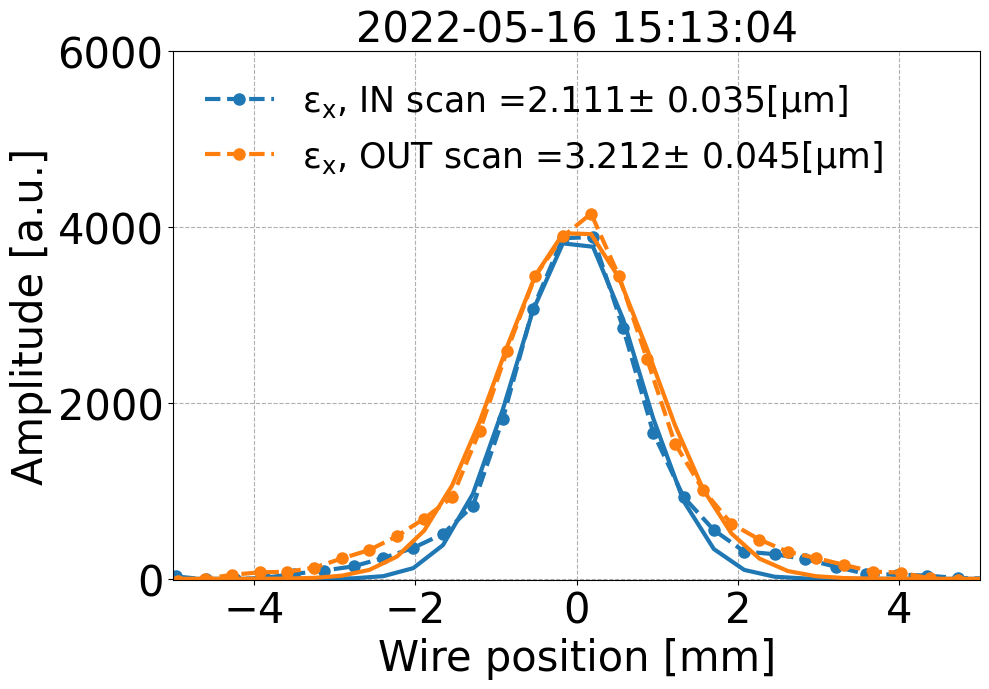
\includegraphics[width=.95\linewidth]{images/app_c/SPS.BWS.51637.H_IN_OUT_ 15_13_04.png}  
        \caption{Horizontal beam profile.}
        \label{fig:WS_example_profiles_H_2022}
    \end{subfigure}
    \begin{subfigure}{.45\textwidth}
        \centering
        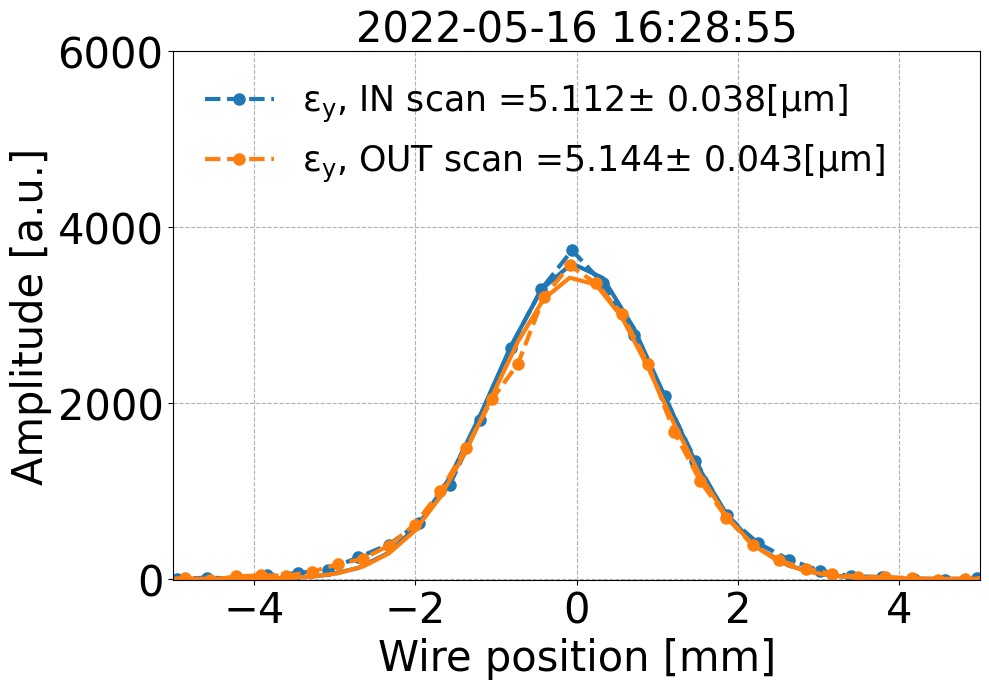
\includegraphics[width=.95\linewidth]{images/app_c/41678.V_IN_OUT_ 16_28_55.png}  
        \caption{Vertical beam profile.}
        \label{fig:WS_example_profiles_V_2022}
    \end{subfigure}
    \caption{Transverse beam profiles as obtained from SPS.BWS.51637.H during the CC experiment in the SPS in 2022. The data points from the IN (OUT) scan are shown with blue (orange) color.}
    \label{fig:WS_example_profiles_H_V_2022}
 \end{figure}

%The emittance values were measured with the SPS Wire Scanners according to the procedure discussed in Section~\ref{subsec:sps_ws}. In particular, wire scanners SPS.BWS.51637.H and SPS.BWS.41677.V were used for measurements in the horizontal and vertical planes, respectively. For both devices the data points from the second photomultiplier were used (PM2)\footnote{Each Wire Scanner device is equipped with four PMs. Each one of them provides a better resolution of the amplitude signal of the secondary particles for a different regime. The choice of PM2 for the emittance growth studies in 2022 was done "online", during the experiment, by examining the obtained beam profiles.}. The beta functions of the respective plane at the locations of the wire scanners are 79.29\,m, and  60.75\,m. 
% The values of the beta functions were obtained from MADX: https://github.com/natriant/exploring_SPS/blob/master/madx_studies/optics_new_seq_after_LS2/output/twiss_thin_elements/find_beta_functions_at_locations.ipynb 



\textbf{IN and OUT scans}\\
As discussed in Section~\ref{subsec:sps_ws}, during each measurement with the Wire Scanners the beam profile is acquired two times as the wire crosses the beam in the forward direction (IN scan) and then in the reverse direction (OUT scan). For the experiment of 2022, the OUT scan was performed just 200\,ms after the IN scan. However, it was observed that there are significant discrepancies between the measurements from IN and OUT scan, which in some cases reached up to 1\,$\mathrm{\mu m}$. By looking at the acquired profiles, e.g. in Fig.~\ref{fig:WS_example_profiles_H_2022} no apparent reason was found to exclude or not one of the two scans.% An example is shown in Fig.~\ref{fig:WS_example_profiles_H_2022}.


A significant effort was done with the Wire Scanner experts during the emittance growth experiment trying to mitigate this effect without success due to limitations on the hardware of the current instrument that still need to be sorted out. Note that this issue was not observed in the 2018 measurements. A possible explanation is that the wire scanner acquisitions of 2022 provide lower number of points to reconstruct the bunch profiles (compare Figs.~\ref{fig:WS_example_V_profile} against~\ref{fig:WS_example_profiles_V_2022}) increasing the uncertainty of the obtained emittances. The reason behind this, is that between 2018 and 2022 the wire scanners had undergone an upgrade which increased their speed while crossing the bunch. A possible solution to this issue would be to reduce the speed of the wire for the emittance growth experiments in coast mode. This is currently in discussion with the team responsible for the Wire Scanners of the SPS. 

For the the SPS $\CC$ tests in 2022, it was decided that the post-process analysis would be performed taking into account only the IN scan measurements since they appeared to have systematically less fluctuation than in the OUT scan. An example is provided in Fig.~\ref{fig:WS_IN_vs_OUT_2022} where it can be seen that the emittance values obtained from the OUT scan appear to be more fluctuated than the values from the IN scan. In this particular example, this is enhanced in the horizontal plane (blue). It is also clearly visible for the acquisitions during the first half of the coast. Furthermore, the acquisitions from the OUT scans leaded to corruputed profiles more frequenly than the IN scans.


%Last, the low emittance growth rates showed a significant sensitivity to the fluctuation of the Wire Scanner measurements. For this reason, for the low $\CC$ noise levels, long measurement times of about 30-40 minutes were needed.



% Evidence for the strong difference between IN and OUT https://docs.google.com/presentation/d/1QIaQNfqVWaI8cHGGgb5eeS7c_jdUMuxLqD_poHrOtH0/edit?usp=sharing

%\textbf{Head-Tail monitor calibration}\\
%From the end of 2018 till the end of 2020, the CERN accelerator complex has undergone its second long shutdown in order to complete its scheduled upgrade program. Therefore, the calibration of the Head-Tail monitor was repeated to provide the normalisation factor required for the scaling of its reading (see Section~\ref{subsec:HT_post_process_CC}). The calibration factor was found to be 0.1037 in November 2021, as shown in Fig.~\ref{fig:HT_calibration_2022_levens} (slope value).

%\begin{figure}[!h] % Email communication with T. Levens on 8 November 2021.
%    \centering         
%    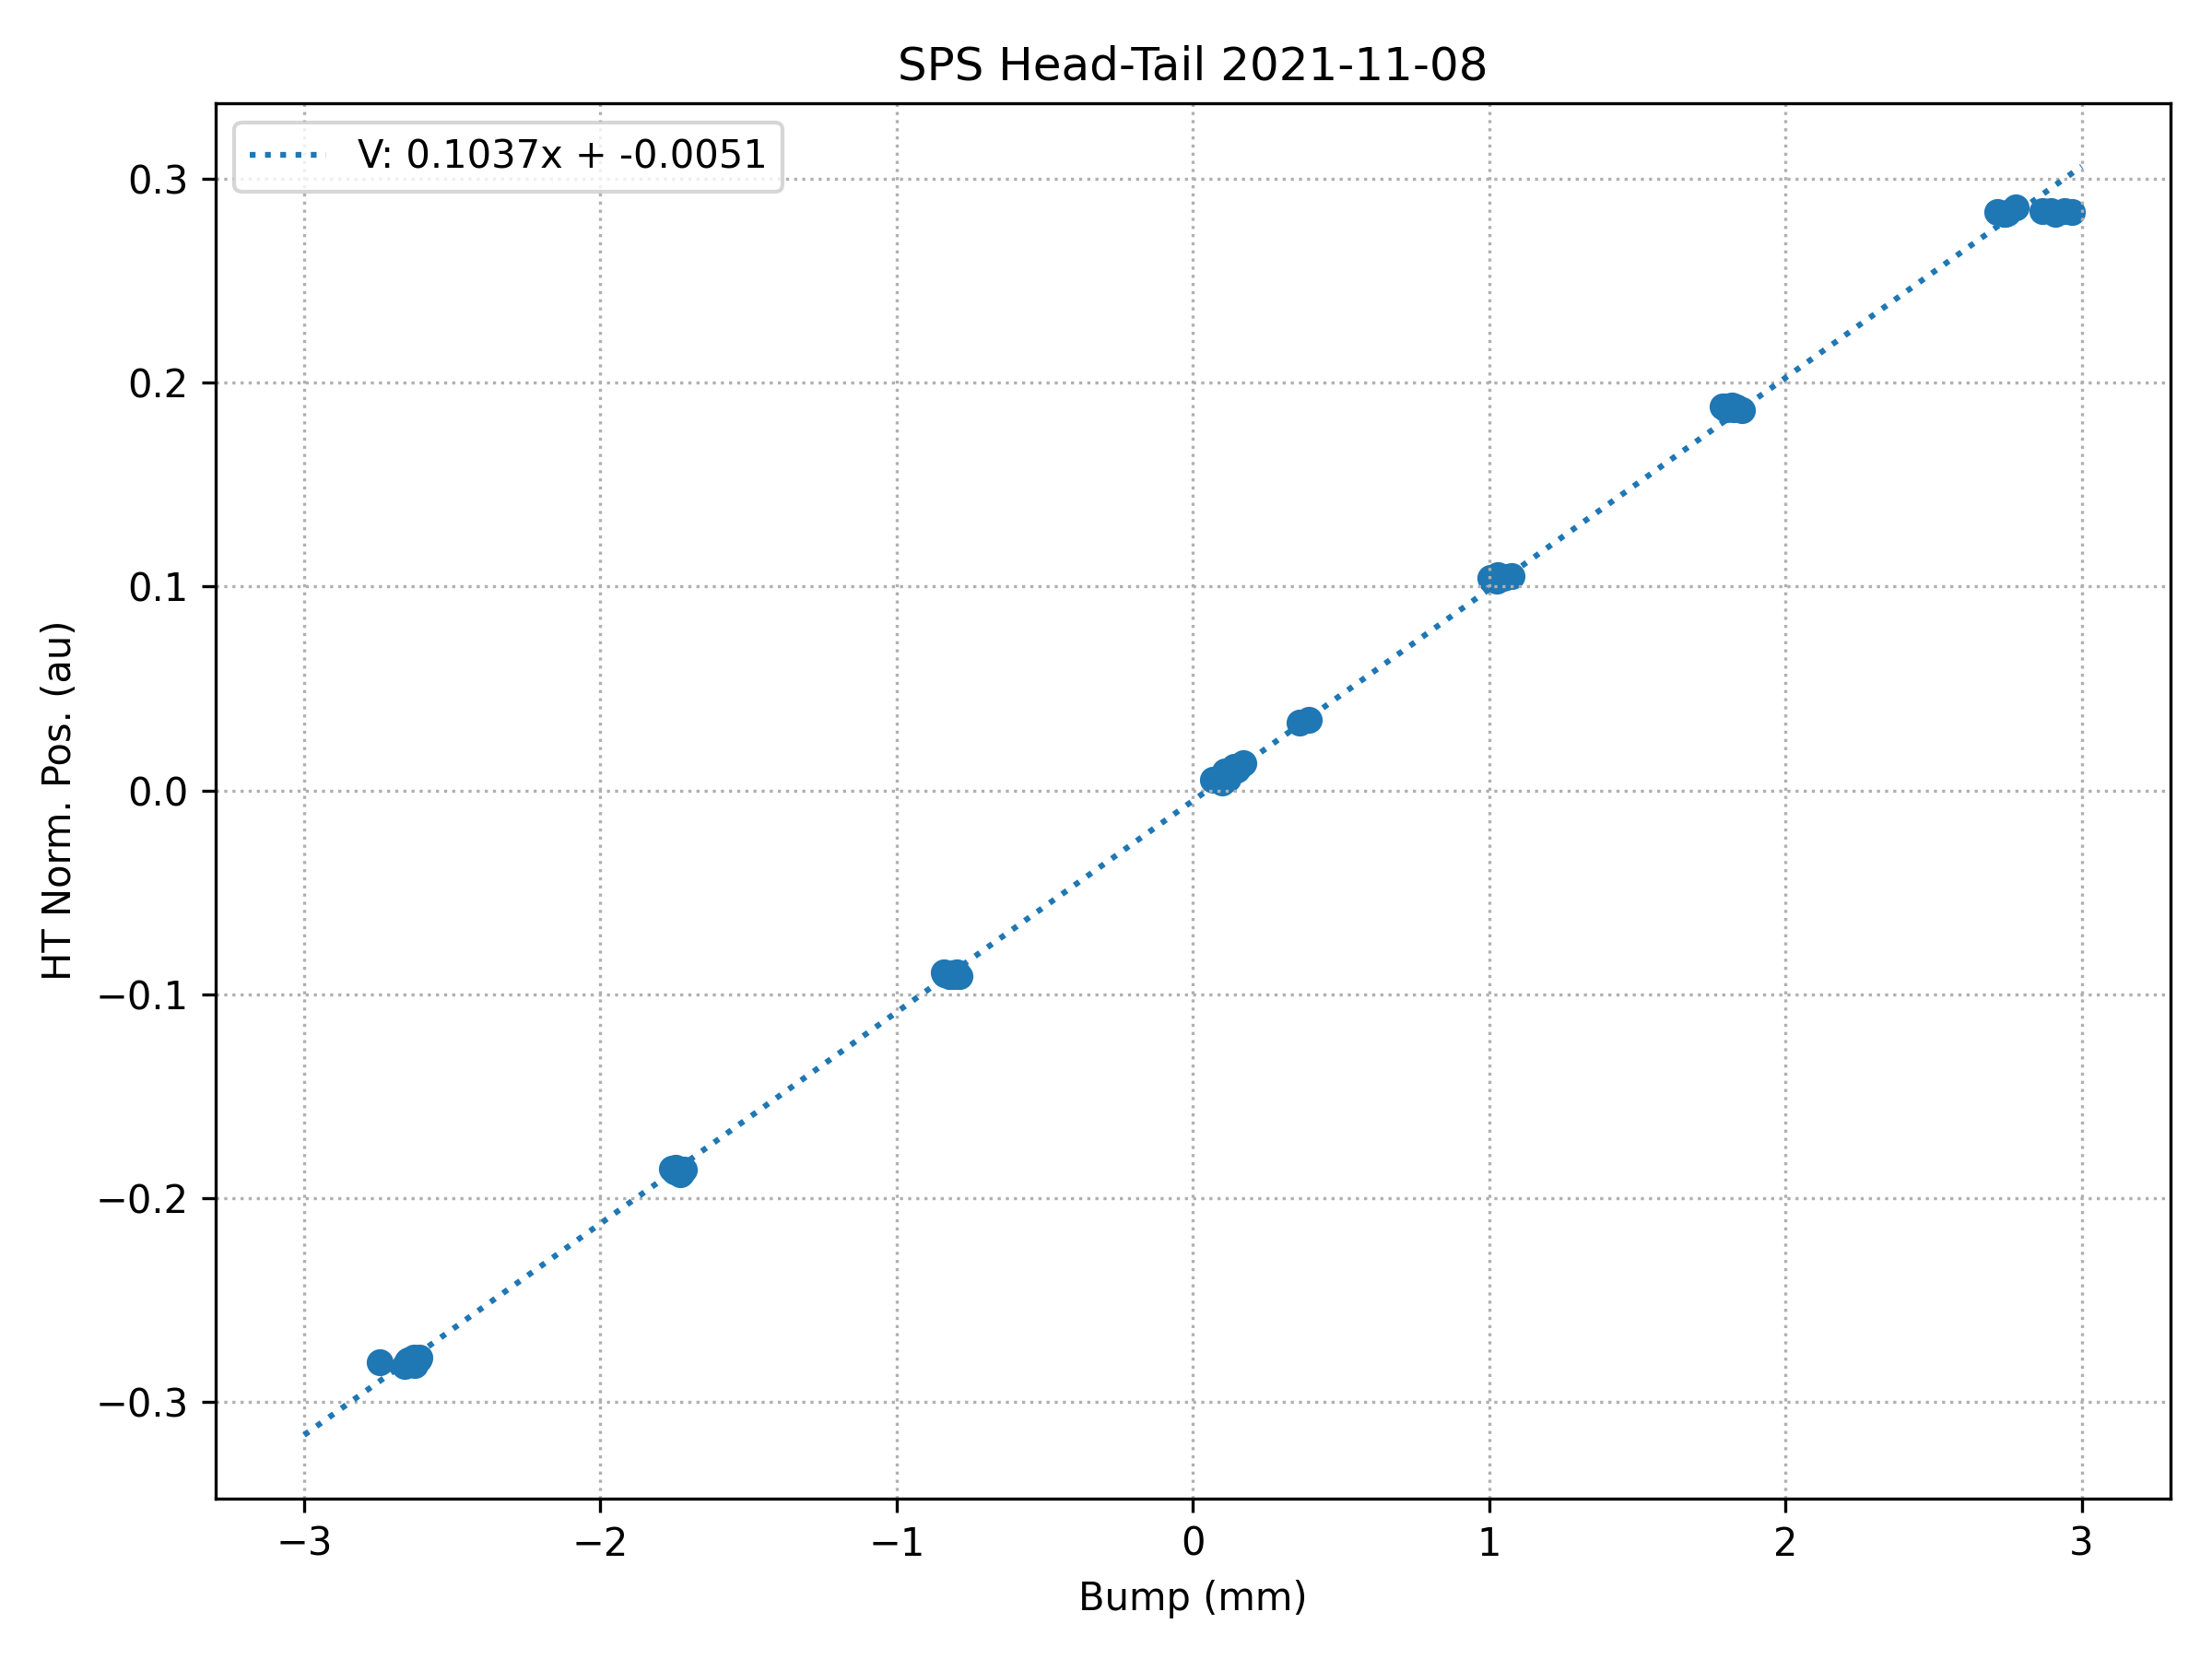
\includegraphics[width=0.7\textwidth]{images/Ch8/HT_monitor_calibration_2022.png}
%        \caption{The calibration was performed by T.~Levens by performing orbit bumps (around the reference orbit) and measuring the normalised position of the bunch in the vertical plane (plane of interest). The normalised position is obtained as the difference of the signal divided by the sum. More details on the calibration procedure are given in~\cite{PhysRevAccelBeams.22.112803}. This plot is courtesy of T.~Levens .}
%        \label{fig:HT_calibration_2022_levens}
% \end{figure}



%\begin{figure}[!h]
 %   \centering         
 %   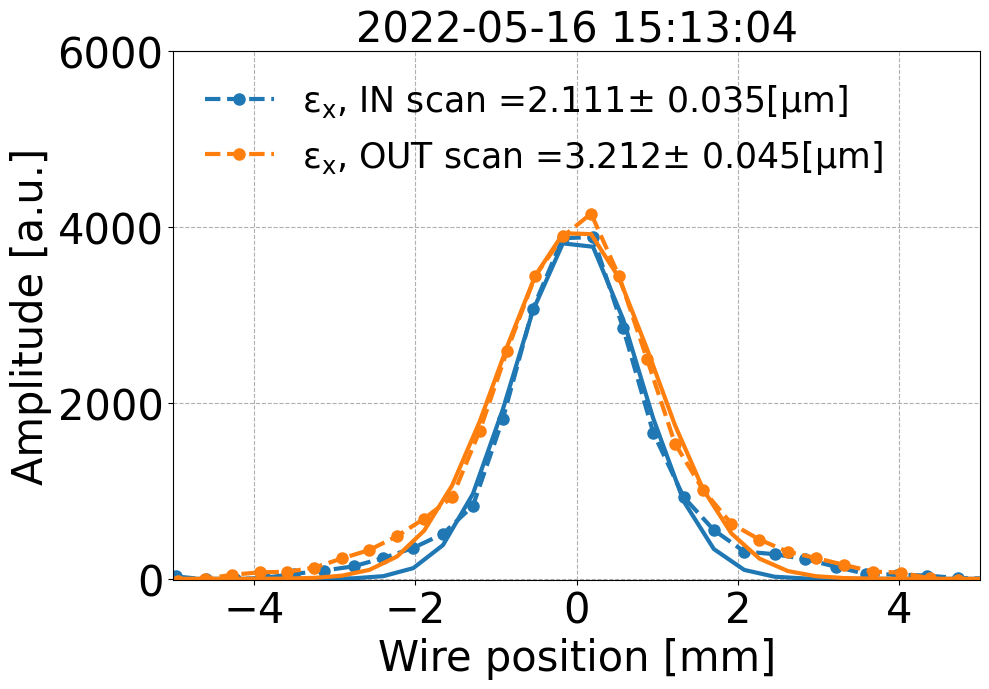
\includegraphics[width=0.6\textwidth]{images/app_c/SPS.BWS.51637.H_IN_OUT_ 15_13_04.png}
 %       \caption{Horizontal beam profile as obtained from SPS.BWS.51637.H during the CC experiment in the SPS in 2022. The data points from the IN (OUT) scan are shown with blue (orange) color. }
%        \label{fig:WS_example_profiles_H_2022}
 %\end{figure}

 %\begin{figure}[!h]
 %   \centering         
 %   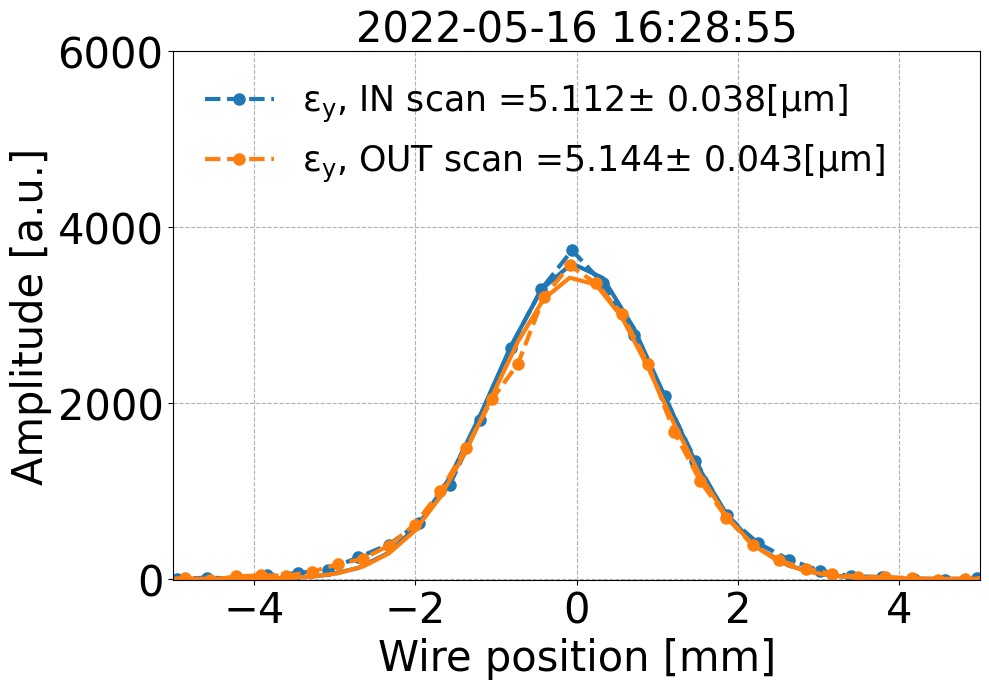
\includegraphics[width=0.6\textwidth]{images/app_c/41678.V_IN_OUT_ 16_28_55.png}
 %       \caption{Vertical beam profile as obtained from SPS.BWS.51637.H during the CC experiment in the SPS in 2022. The data points from the IN (OUT) scan are shown with blue (orange) color. }
 %       \label{fig:WS_example_profiles_V_2022}
 %\end{figure}

 %\subsection{Emittance values from IN and OUT scan}\label{subsec:ex_emit_growth_in_vs_out}
 %Figure~\ref{fig:WS_IN_vs_OUT_2022} shows the transverse emittance evolution acquired with  SPS.BWS.51637.H and SPS.BWS.41677.V for horizontal and vertical planes respectively during the experiment with CC noise on May 16, 2022. The emittance values acquired during the IN scan are shown on the left while the ones acquired during the OUT scan are shown on the right. 

%It can be seen that the emittance values obtained from the OUT scan appear to be more fluctuated than the values from the IN scan. In this particular example, this is enhanced in the horizontal plane (blue). It is also clearly visible for the acquisitions during the first half of the coast.

% Path to data:/eos/user/n/natriant/2022/SPS_MDs_2022/cc_md_16May2022/roundA_online_analysis_ws/for_thesis/coast8
% Relevant slides: https://docs.google.com/presentation/d/1QIaQNfqVWaI8cHGGgb5eeS7c_jdUMuxLqD_poHrOtH0/edit#slide=id.g148272a84c8_2_0
 \begin{figure}[htp]
    \centering
    \begin{subfigure}{.45\textwidth}
        \centering
        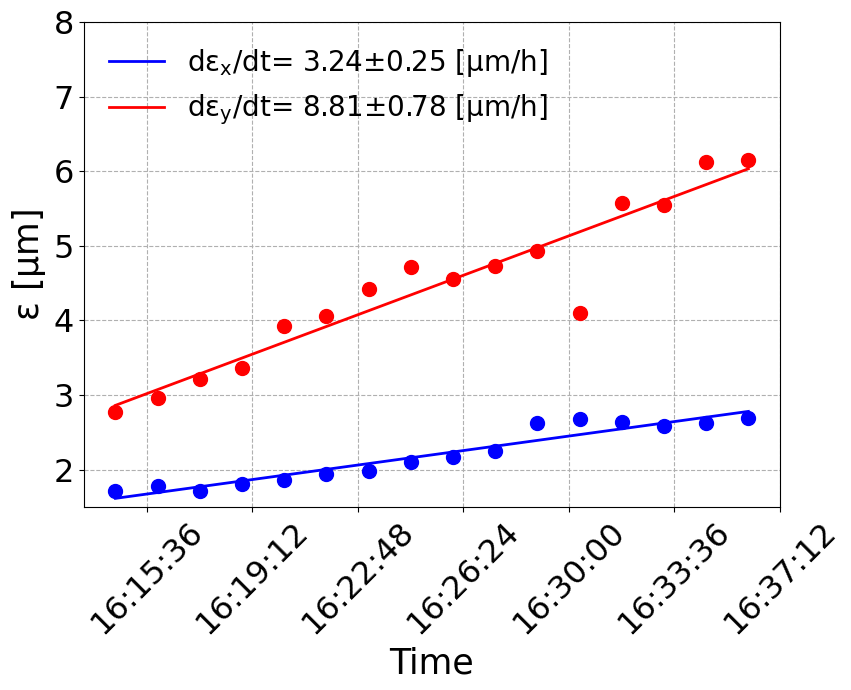
\includegraphics[width=.95\linewidth]{images/app_c/ws_coast8_set1.png}  
        \caption{Emittance evolution from IN scan.}
        \label{fig:WS_example_profiles_H_2022}
    \end{subfigure}
    \begin{subfigure}{.45\textwidth}
        \centering
        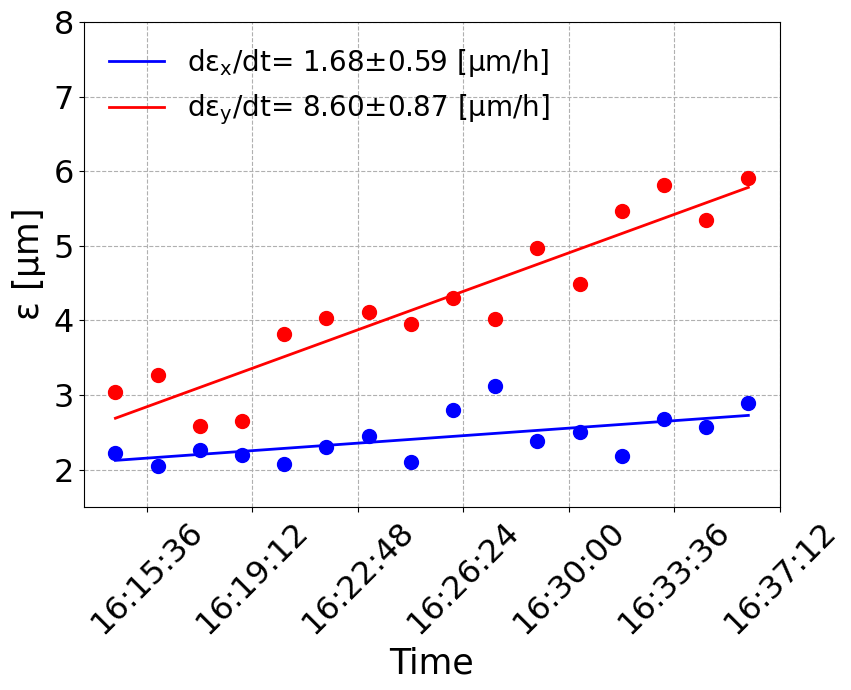
\includegraphics[width=.95\linewidth]{images/app_c/ws_coast8_set2.png}  
        \caption{Emittance evolution from OUT scan.}
        \label{fig:WS_example_profiles_V_2022}
    \end{subfigure}
    \caption{Transverse beam profiles as obtained from SPS.BWS.51637.H during the CC experiment in the SPS in 2022. The data points from the IN (OUT) scan are shown with blue (orange) color.}
    \label{fig:WS_IN_vs_OUT_2022}
 \end{figure}

\newpage
 \section{Transverse emittance growth measurements}\label{sec:emittance_growth_2022}

In this section, the individual emittance growth measurements for each coast of the from the SPS $\CC$ tests that were conduced in 2022 are presented.


 \subsection{Experiment II: sensitivity of emittance growth to amplitude-dependent tune shift}\label{subsec:emittance_growth_2022_exper2}


% location: /eos/user/n/natriant/2022/SPS_MDs_2022/cc_md_16May2022/roundA_online_analysis_ws/for_thesis
% script to plot: /afs/cern.ch/work/n/natriant/public/SPS_MDs_2022/cc_md_16May2022/ws_measurements 
\begin{figure}[h!]
    \centering
    \begin{subfigure}{.45\textwidth}
        \centering
        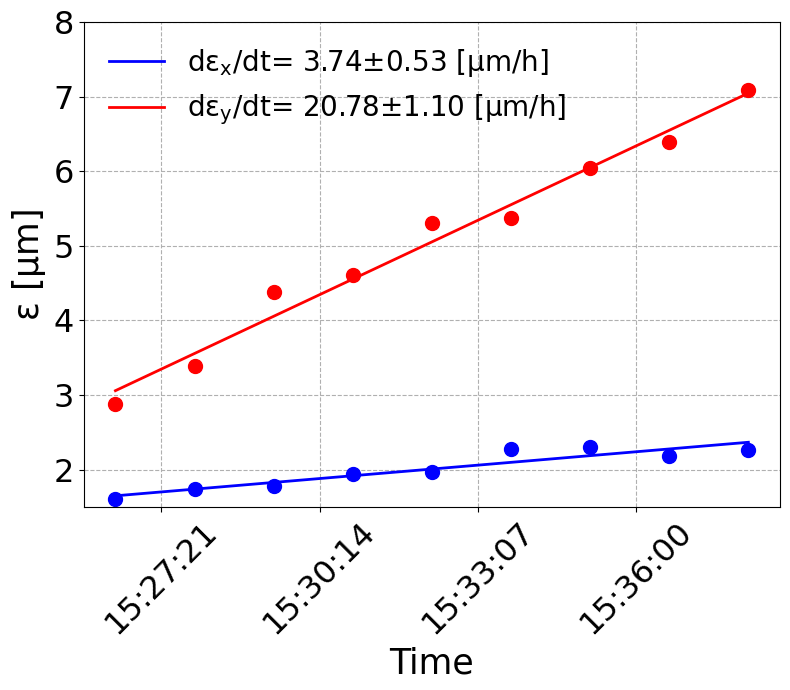
\includegraphics[width=.95\linewidth]{images/Ch8/emit_vs_time_Set1_coast6.png}  
        \caption{$k_\mathrm{LOD}=+15 \ \mathrm{/m^{4}}$}
        \label{fig:cc_md_2022_coast6}
    \end{subfigure}
    \begin{subfigure}{.45\textwidth}
        \centering
        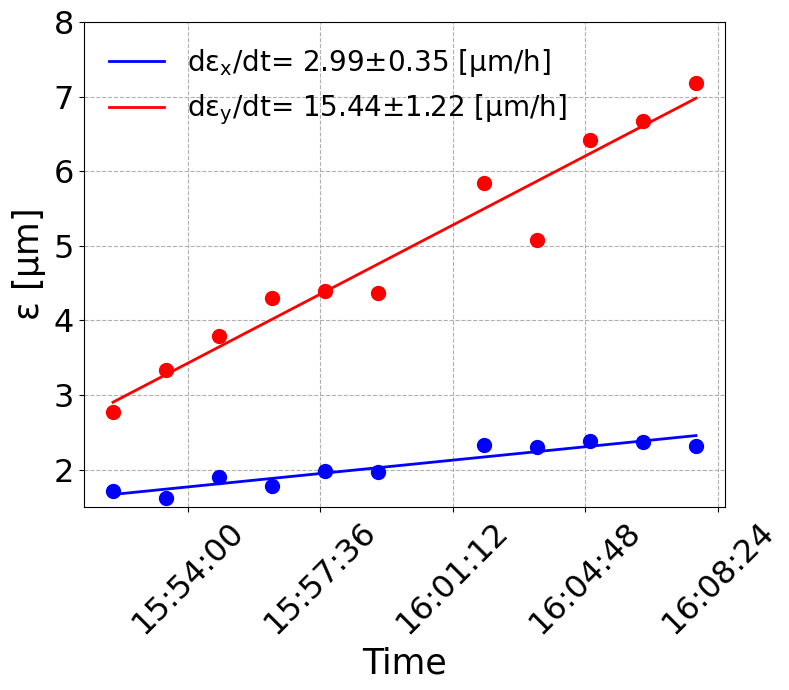
\includegraphics[width=.95\linewidth]{images/Ch8/emit_vs_time_Set1_coast7.png}  
        \caption{$k_\mathrm{LOD}=+10 \ \mathrm{/m^{4}}$}
        \label{fig:cc_md_2022_coast7}
    \end{subfigure}
    \begin{subfigure}{.45\textwidth}
        \centering
        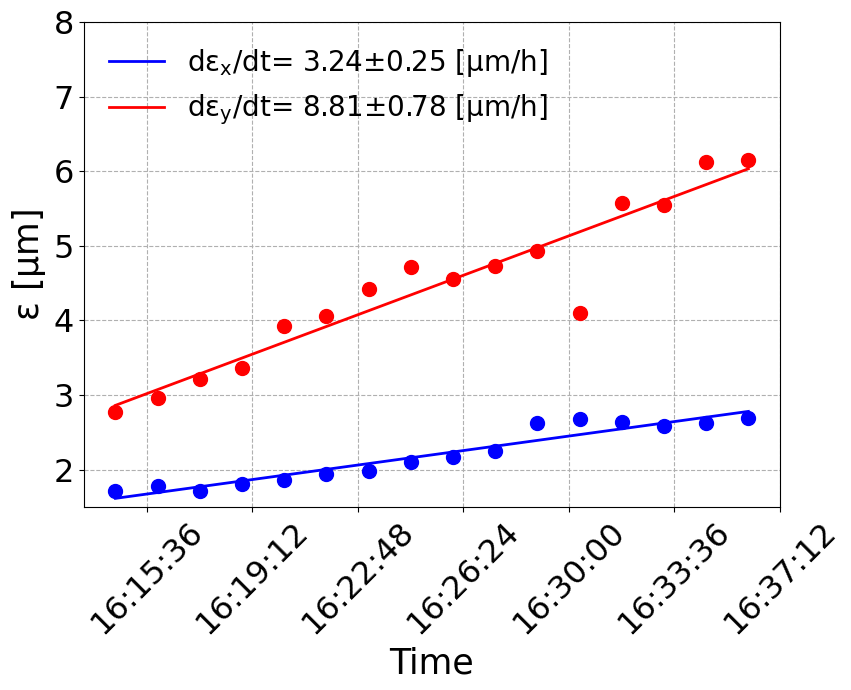
\includegraphics[width=.95\linewidth]{images/Ch8/emit_vs_time_Set1_coast8.png}  
        \caption{$k_\mathrm{LOD}=+5 \ \mathrm{/m^{4}}$}
        \label{fig:cc_md_2022_coast8}
    \end{subfigure}
    \begin{subfigure}{.45\textwidth}
            \centering
            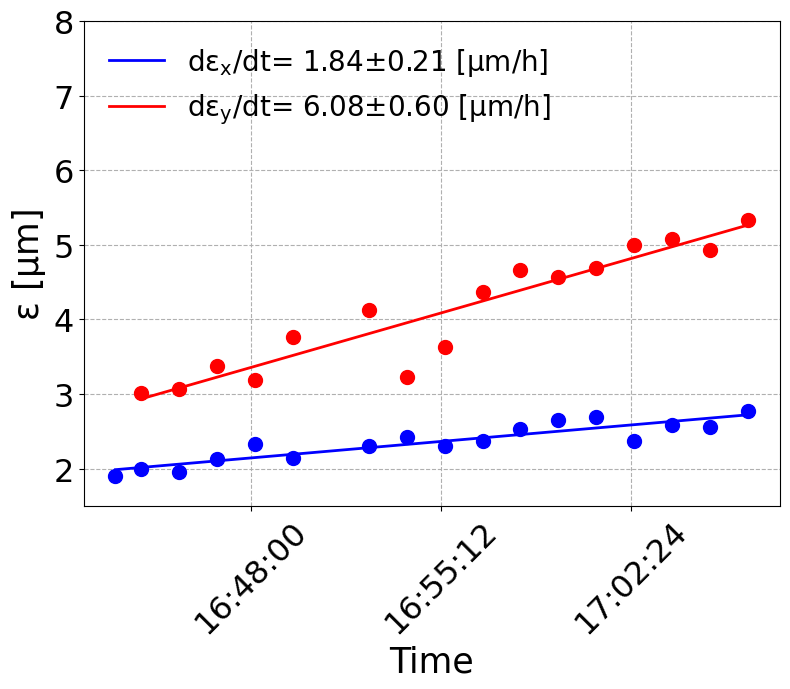
\includegraphics[width=.95\linewidth]{images/Ch8/emit_vs_time_Set1_coast9.png}  
            \caption{$k_\mathrm{LOD}=-5 \ \mathrm{/m^{4}}$}
            \label{fig:cc_md_2022_coast9}
    \end{subfigure}
    \caption{Horizontal (blue) and vertical (red) emittance evolution of a single bunch during the CC experiment on 16 May, 2022 driven by phase noise of -104.7\,dBc/Hz. The different octupole settings are displayed in the captions of each plot.}
    \label{fig:cc_md_2022_overview_plots_klod_scan}
 \end{figure}
 
 \newpage
 \subsection{Experiment III: emittance growth measurements in the presence of strong octupoles}\label{subsec:emit_growth_cc_md_sep2022}

 %The individual measurements of the transverse emittance evolution for each octupole setting during the experiment with $\CC$ RF noise that took place on September 12, 2022, are illustrated in Fig.~\ref{fig:cc_md_12sep2022_overview_plots_klod_scan}. The subplots are plotted in chronological order. The measurements were conducted with artifical noise injected in the $\CC$ RF system which was a mixture of amplitude and phase noise. The amplitude and phase noise level at the betatron frequency were measured to be -123.3\,dBc/Hz and -103.3\,dBc/Hz respectively. %The measurements were done with a spectrum analyzer connected directly to the $\CC$ antena.
 
 % Location of figures: /eos/user/n/natriant/2022/SPS_MDs_2022/cc_md_12Sep2022/ws_emittance_growth/figures_for_thesis
 % Plotting sctipt: /eos/user/n/natriant/2022/SPS_MDs_2022/cc_md_12Sep2022/ws_emittance_growth/plot_emitGrowth_vs_time_for_thesis.py. But I run it in afs in my public location
 \begin{figure}[htp]
    \centering
    \begin{subfigure}{.4\textwidth}
        \centering
        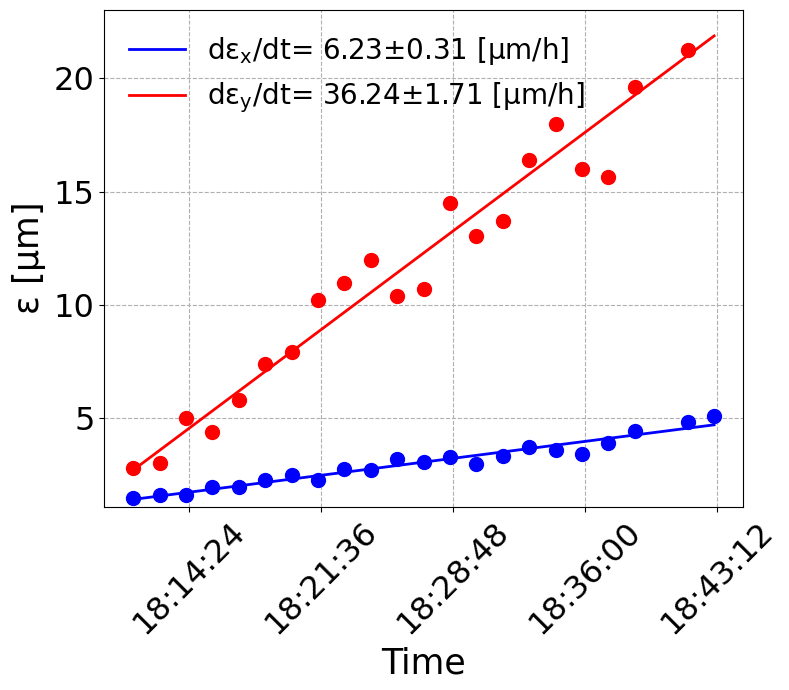
\includegraphics[width=.95\linewidth]{images/app_c/cc_md_12sep22_coast6.png}  
        \caption{$k_\mathrm{LOD}=-30 \mathrm{/m^{4}}$}
    \end{subfigure}
    \begin{subfigure}{.4\textwidth}
        \centering
        \includegraphics[width=.95\linewidth]{images/app_c/cc_md_12sep22_coast7.png}  
        \caption{$k_\mathrm{LOD}=-20 \mathrm{/m^{4}}$}
    \end{subfigure}
    \begin{subfigure}{.4\textwidth}
        \centering
        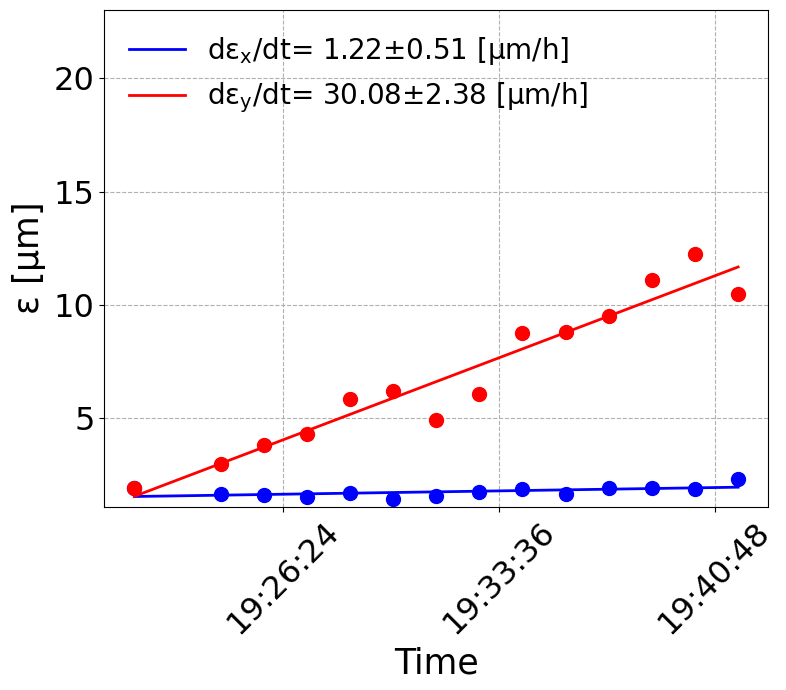
\includegraphics[width=.95\linewidth]{images/app_c/cc_md_12sep22_coast8.png}  
        \caption{$k_\mathrm{LOD}=-10  \mathrm{/m^{4}}$}
    \end{subfigure}
    \begin{subfigure}{.4\textwidth}
            \centering
            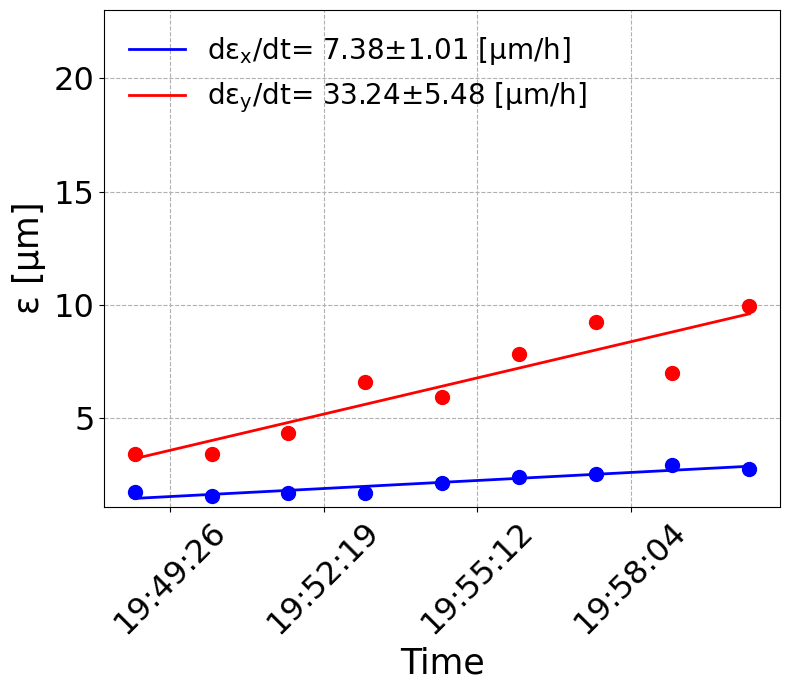
\includegraphics[width=.95\linewidth]{images/app_c/cc_md_12sep22_coast9.png}  
            \caption{$k_\mathrm{LOD}=+30  \mathrm{/m^{4}}$}
    \end{subfigure}
    \begin{subfigure}{.4\textwidth}
        \centering
        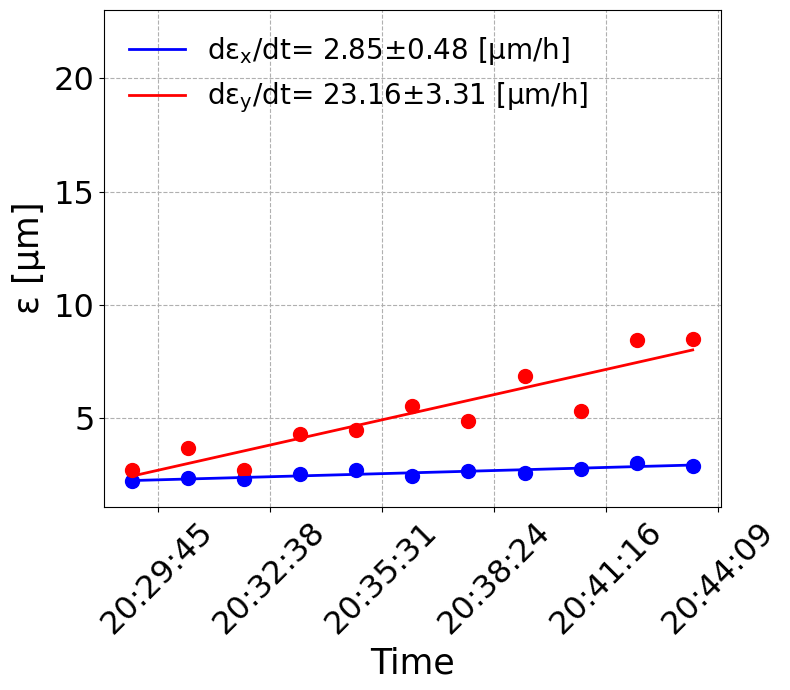
\includegraphics[width=.95\linewidth]{images/app_c/cc_md_12sep22_coast11.png}  
        \caption{$k_\mathrm{LOD}=+10 \mathrm{/m^{4}}$}
    \end{subfigure}
    \caption{Horizontal (blue) and vertical (red) emittance evolution of a single bunch during the experiment with dipole noise on September 12, 2022.  The different octupole settings are displayed at the captions of each plot.}
    \label{fig:cc_md_12sep2022_overview_plots_klod_scan}
 \end{figure}
 
\newpage
 \subsection{Experiment V: emittance growth driven by dipole noise}\label{subsec:exp5_coast_md_damper_2022_emittance}
 %The individual measurements of the transverse emittance evolution for each octupole setting during the experiment with dipole noise are illustrated in Fig.~\ref{fig:dipole_noise_md_2022_overview_plots_klod_scan}. The subplots are plotted in chronological order.

% Notes on the MD: https://docs.google.com/document/d/1b8fRJA5DN0hczIx2_O1NQzwV8dgKYmrJCmZzmH3qBn0/edit
% Path to figures: /eos/user/n/natriant/2022/SPS_MDs_2022/coast_md_damper_16May2022/coast_plots_for_thesis
% Plotting script: /afs/cern.ch/work/n/natriant/public/SPS_MDs_2022/coast_16May2022_damper/ws_measurements

\begin{figure}[htp]
    \centering
    \begin{subfigure}{.45\textwidth}
        \centering
        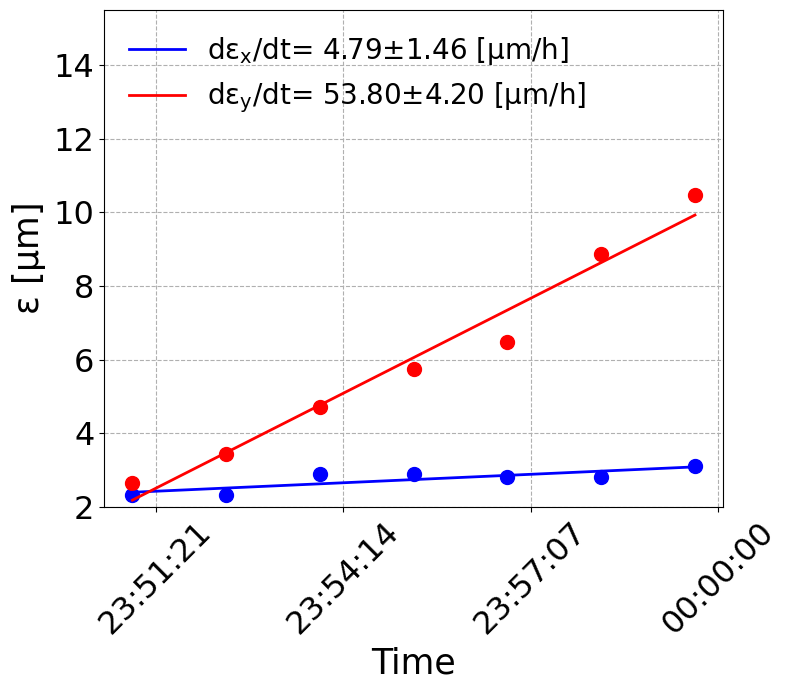
\includegraphics[width=.95\linewidth]{images/app_c/emit_vs_time_Set1_coast1.png}  
        \caption{$k_\mathrm{LOD}=+15 \mathrm{/m^{4}}$}
    \end{subfigure}
    \begin{subfigure}{.45\textwidth}
        \centering
        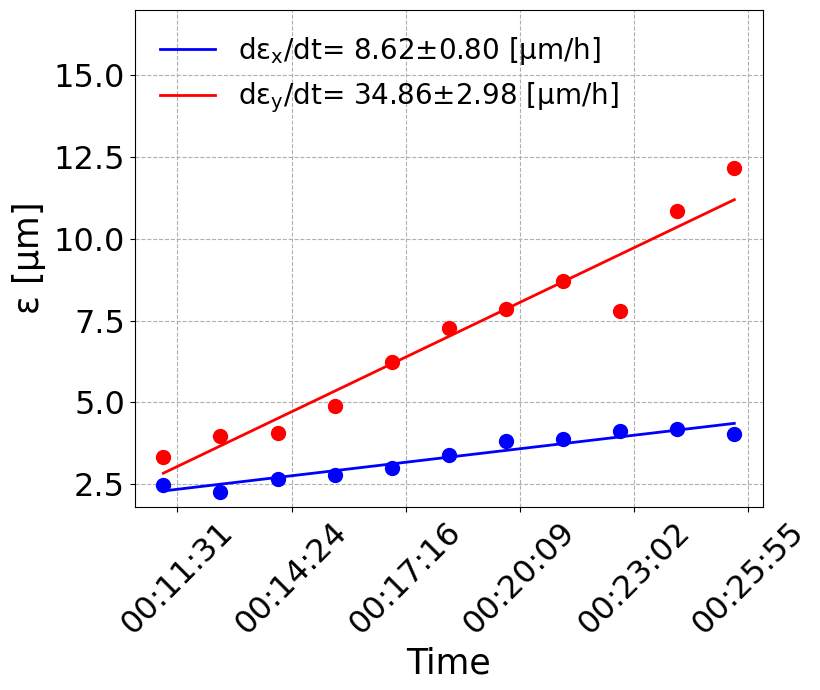
\includegraphics[width=.95\linewidth]{images/app_c/emit_vs_time_Set1_coast2.png}  
        \caption{$k_\mathrm{LOD}=+10 \mathrm{/m^{4}}$}
    \end{subfigure}
    \begin{subfigure}{.45\textwidth}
        \centering
        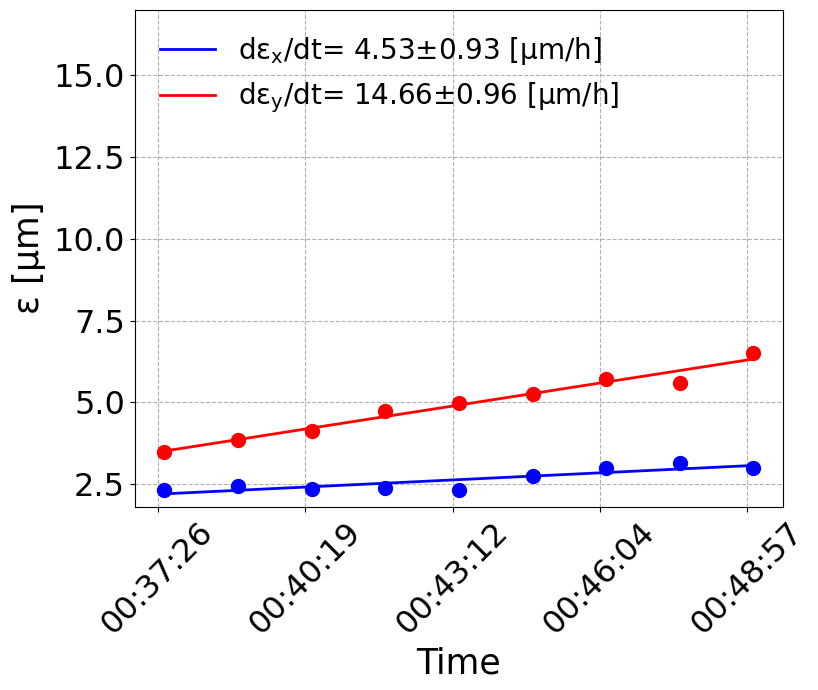
\includegraphics[width=.95\linewidth]{images/app_c/emit_vs_time_Set1_coast3.png}  
        \caption{$k_\mathrm{LOD}=+5  \mathrm{/m^{4}}$}
    \end{subfigure}
    \begin{subfigure}{.45\textwidth}
            \centering
            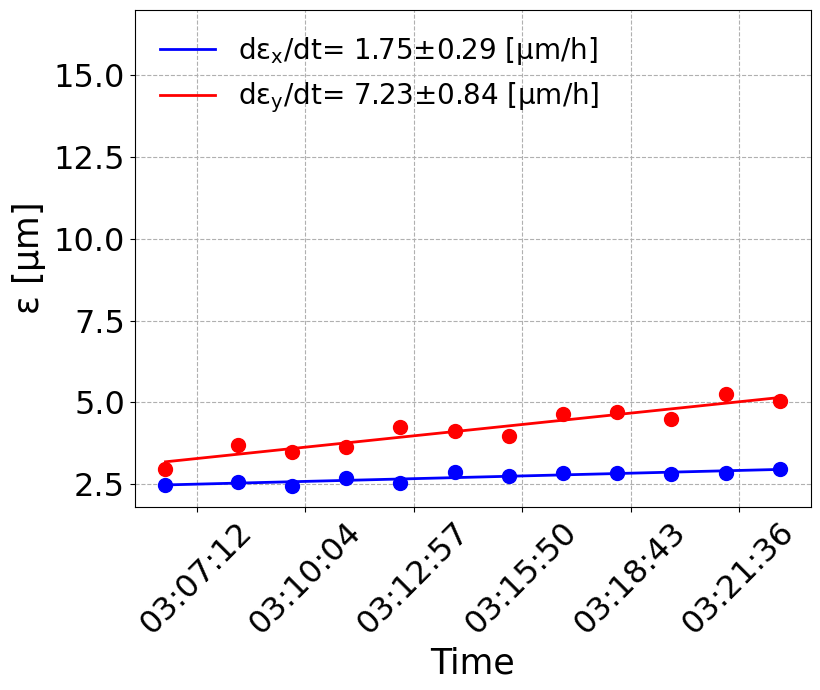
\includegraphics[width=.95\linewidth]{images/app_c/emit_vs_time_Set1_coast4.png}  
            \caption{$k_\mathrm{LOD}=0  \mathrm{/m^{4}}$}
    \end{subfigure}
    \begin{subfigure}{.45\textwidth}
        \centering
        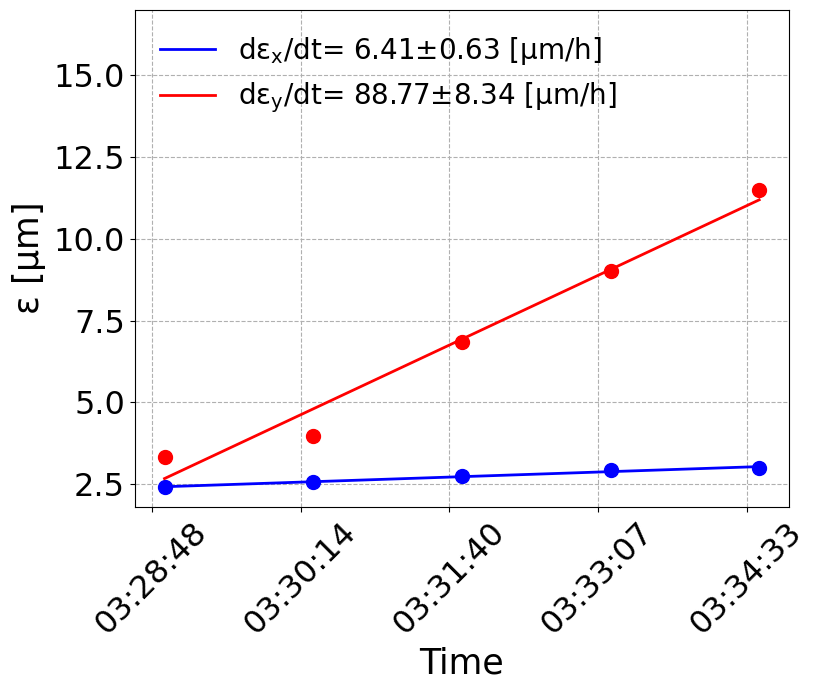
\includegraphics[width=.95\linewidth]{images/app_c/emit_vs_time_Set1_coast5.png}  
        \caption{$k_\mathrm{LOD}=-15  \mathrm{/m^{4}}$}
    \end{subfigure}
    \begin{subfigure}{.45\textwidth}
            \centering
            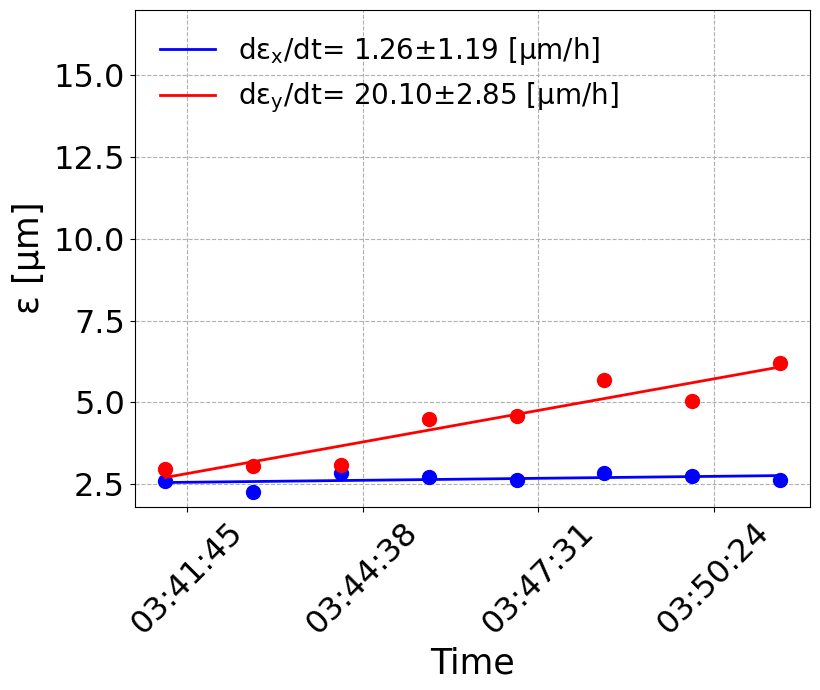
\includegraphics[width=.95\linewidth]{images/app_c/emit_vs_time_Set1_coast6.png}  
            \caption{$k_\mathrm{LOD}=-7.5  \mathrm{/m^{4}}$}
    \end{subfigure}
    \begin{subfigure}{.45\textwidth}
        \centering
        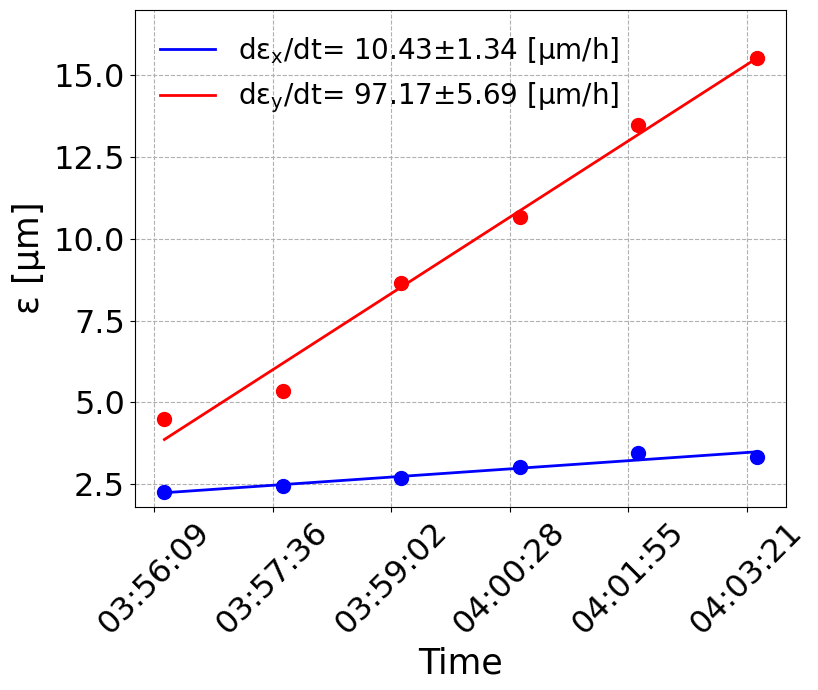
\includegraphics[width=.95\linewidth]{images/app_c/emit_vs_time_Set1_coast7.png}  
        \caption{$k_\mathrm{LOD}=+25  \mathrm{/m^{4}}$}
\end{subfigure}
    \caption{Horizontal (blue) and vertical (red) emittance evolution of a single bunch during the experiment with dipole noise on May 16-17, 2022.  The different octupole settings are displayed at the captions of each plot.}
    \label{fig:dipole_noise_md_2022_overview_plots_klod_scan}
 \end{figure}
 
 
\newpage
 \section{Bunch length measurements}\label{sec:bunch_length_meas_2022}
 The bunch length measurements presented in this section were performed with the Wall Current Monitor (WCM). The WCM acquires the longitudinal bunch profiles which are fitted with a Gaussian function in the post-processing for the evaluation of the bunch length. Each data point shown in the folllowing plots corresponds to the average bunch length value obtained from 100 subsequent acquisitions, while the error bars indicate the standard deviation.

 Further details on the WCM that are installed in the CERN Proton Synchrotron (PS) and Large Hadron Collider (LHC) can be found in~\cite{Belleman:2313362, Argyropoulos:2752314}. The device installed in the SPS follows the same working principle. 


 %https://accelconf.web.cern.ch/e08/papers/thpc144.pdf (from email communication with IVAN)
 

\newpage
 \subsection{Experiment I: dependece of emittance growth on CC RF noise power}\label{subsec:2022_exp1_bunch_length}
 %Figure~\ref{fig:cc_md_2022_overview_plots_noise_scan_bunch_length} illustrates the evolution of the rms bunch length measured in the SPS on May 16, 2022, for the four different levels of phase noise injected in the CC RF system increasing from the top left to bottom right. The Wall Current monitor acquires the longitudinal bunch profiles, from which the bunch length is computed, once per turn. In the figures below, each point corresponds to the average bunch lengths from the profiles over 100 turns while the error bars indicate the standard deviation between them. \textcolor{red}{Is it correct that is acquires profiles once per turn?}
 % Scripting plot: /eos/user/n/natriant/2022/SPS_MDs_2022/cc_md_16May2022/longitudinal_profiles/plot_bunch_length_for_thesis.ipynb
 \begin{figure}[htp]
     \centering
     \begin{subfigure}{.45\textwidth}
         \centering
         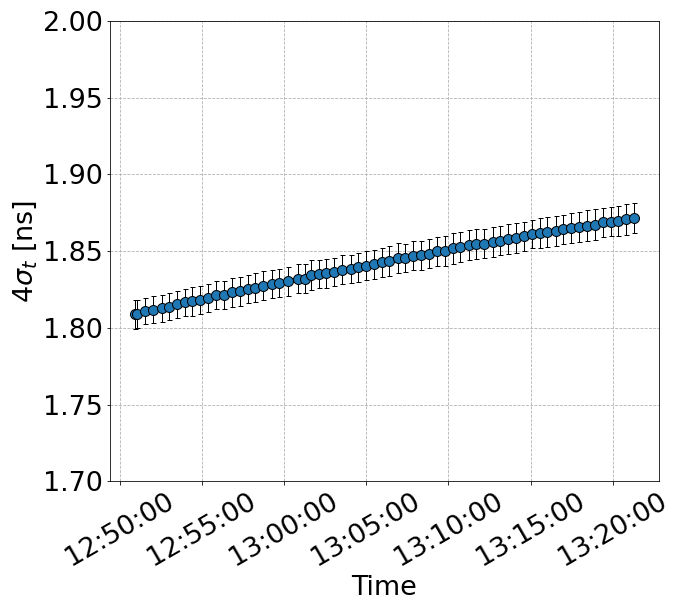
\includegraphics[width=.95\linewidth]{images/app_c/bunch_length_COAST_02.png}  
         \caption{-115.2\,dBc/Hz}
         %\label{fig:cc_md_2022_coast2}
     \end{subfigure}
     \begin{subfigure}{.45\textwidth}
         \centering
         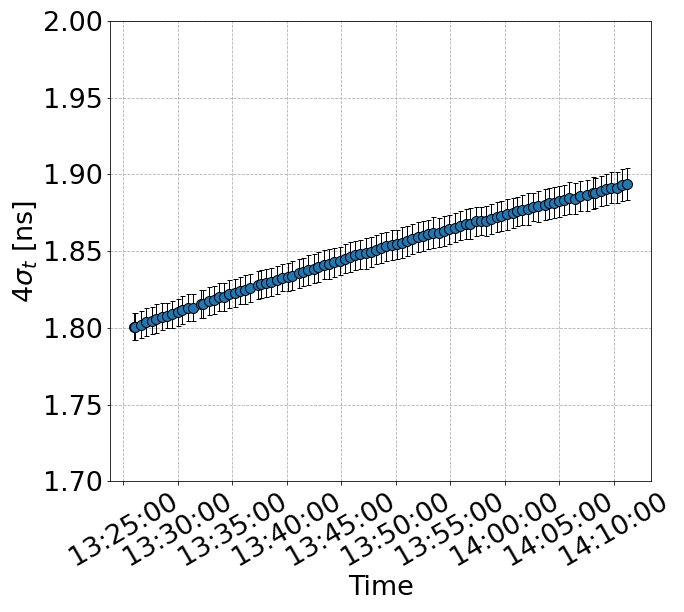
\includegraphics[width=.95\linewidth]{images/app_c/bunch_length_COAST_03.png}  
         \caption{-109.5\,dBc/Hz}
         %\label{fig:cc_md_2022_coast3}
     \end{subfigure}
     \begin{subfigure}{.45\textwidth}
         \centering
         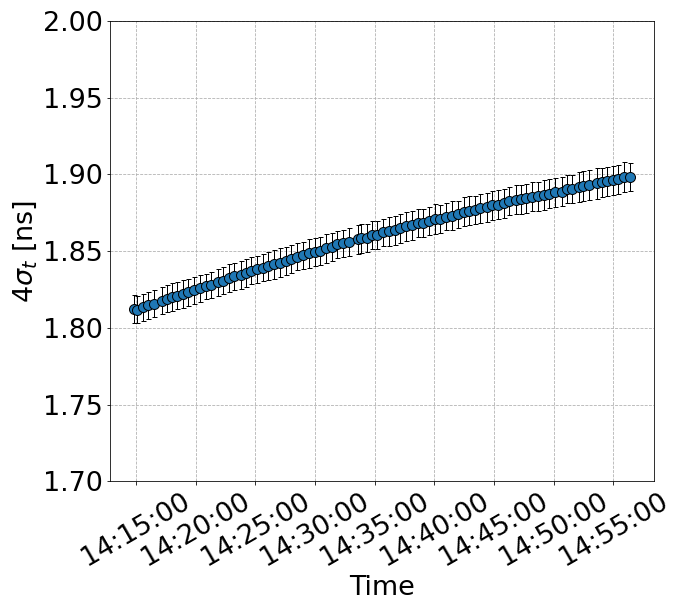
\includegraphics[width=.95\linewidth]{images/app_c/bunch_length_COAST_04.png}  
         \caption{-104.7\,dBc/Hz}
         %\label{fig:cc_md_2022_coast4}
     \end{subfigure}
     \begin{subfigure}{.45\textwidth}
             \centering
             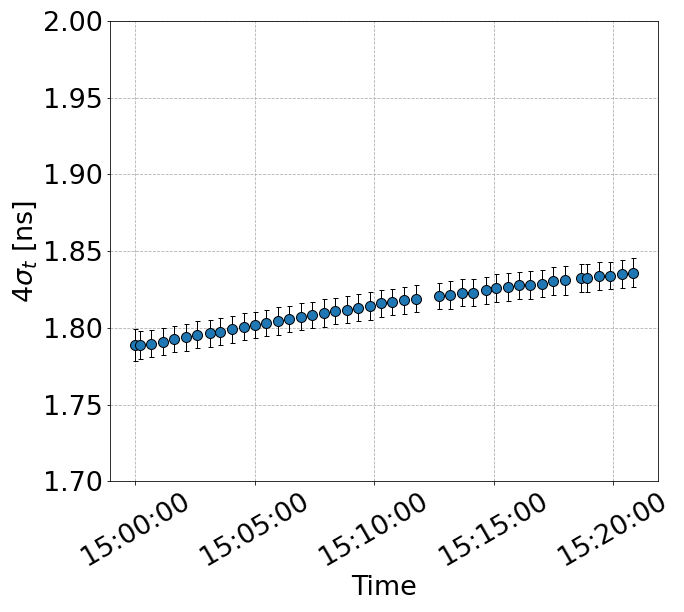
\includegraphics[width=.95\linewidth]{images/app_c/bunch_length_COAST_05.png}  
             \caption{-100.1\,dBc/Hz}
             %\label{fig:cc_md_2022_coast5}
     \end{subfigure}
     \caption{Evolution of the bunch length during the CC Experiment I on May 16, 2022. The different phase noise levels injected in the RF system of CC1, are displayed at the captions of each plot.}
     \label{fig:cc_md_2022_overview_plots_noise_scan_bunch_length}
  \end{figure}
  
  \newpage


 \subsection{Experiment II: sensitivity of emittance growth to amplitude-dependent tune shift}\label{subsec:2022_exp2_bunch_length}

 % Scripting plot: /eos/user/n/natriant/2022/SPS_MDs_2022/cc_md_16May2022/longitudinal_profiles/plot_bunch_length_for_thesis.ipynb
  \begin{figure}[htp]
     \centering
     \begin{subfigure}{.45\textwidth}
         \centering
         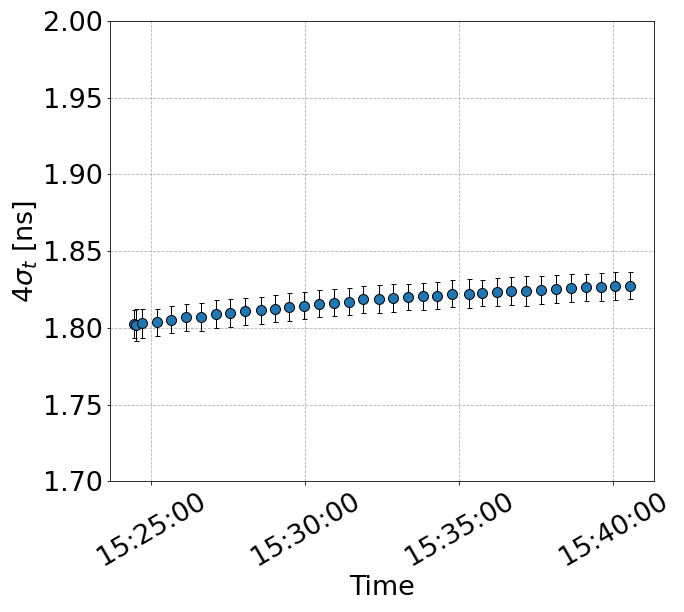
\includegraphics[width=.95\linewidth]{images/app_c/bunch_length_COAST_06.png}  
         \caption{$k_\mathrm{LOD}=+15 \mathrm{/m^{4}}$}
         %\label{fig:cc_md_2022_coast6}
     \end{subfigure}
     \begin{subfigure}{.45\textwidth}
         \centering
         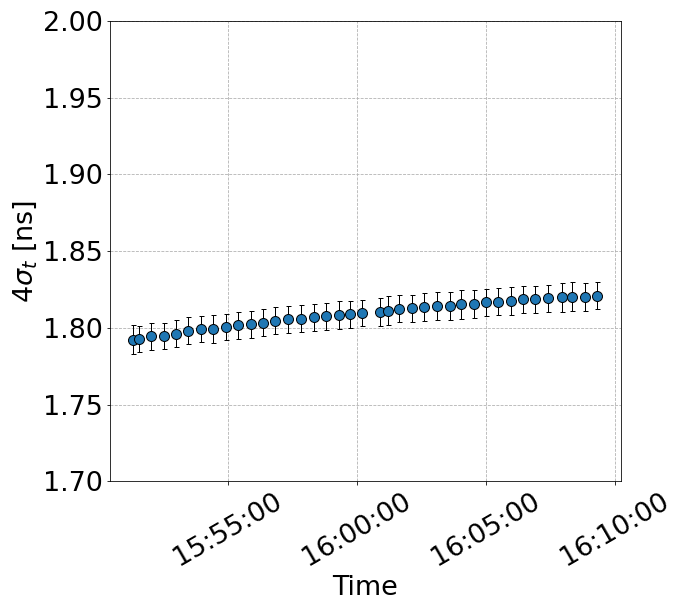
\includegraphics[width=.95\linewidth]{images/app_c/bunch_length_COAST_07.png}  
         \caption{$k_\mathrm{LOD}=+10  \mathrm{/m^{4}}$}
         %\label{fig:cc_md_2022_coast7}
     \end{subfigure}
     \begin{subfigure}{.45\textwidth}
         \centering
         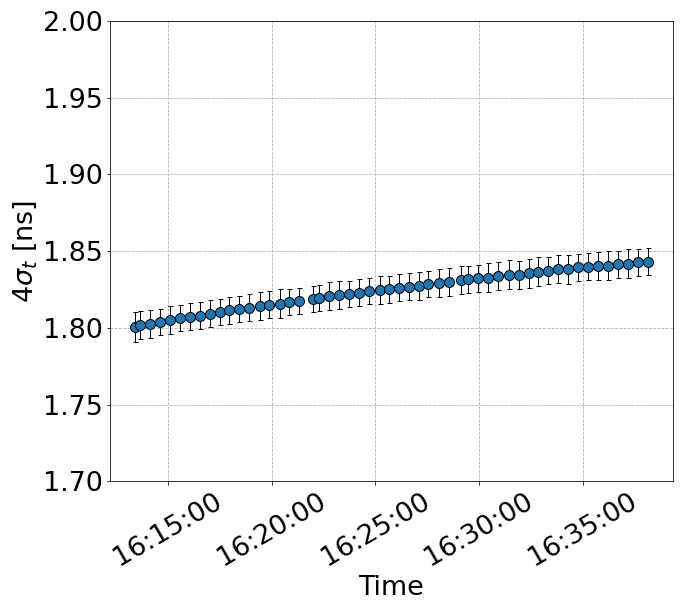
\includegraphics[width=.95\linewidth]{images/app_c/bunch_length_COAST_08.png}  
         \caption{$k_\mathrm{LOD}=+5  \mathrm{/m^{4}}$}
         %\label{fig:cc_md_2022_coast8}
     \end{subfigure}
     \begin{subfigure}{.45\textwidth}
             \centering
             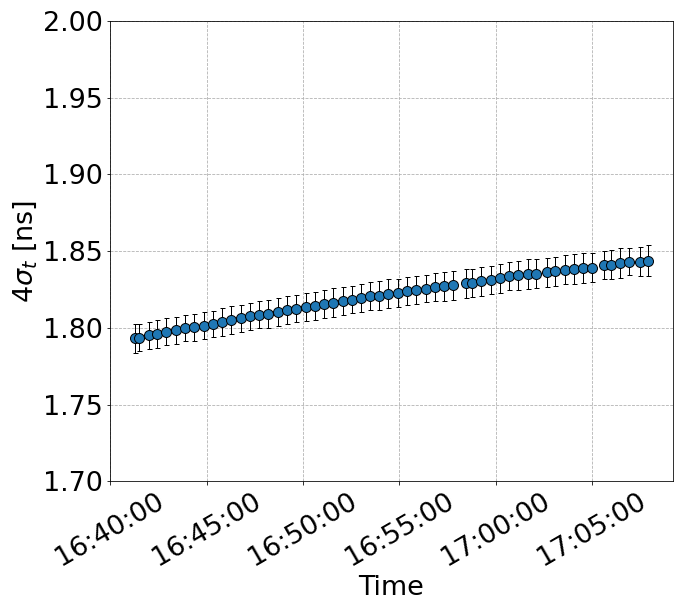
\includegraphics[width=.95\linewidth]{images/app_c/bunch_length_COAST_09.png}  
             \caption{$k_\mathrm{LOD}=-5 \mathrm{/m^{4}}$}
             %\label{fig:cc_md_2022_coast9}
     \end{subfigure}
     \caption{Evolution of the bunch length during the  CC Experiment II on May 16, 2022. The different octupole settings are displayed at the captions of each plot.}
     \label{fig:cc_md_2022_overview_plots_klod_scan_bunch_length}
  \end{figure}
 
 
 The average measured bunch length over all above coasts on May 16, 2022 (Experiments I and II) was found to be, 4$\sigma_t$=1.83\,ns. 
 
 \newpage
 

 \subsection{Experiment III: emittance growth measurements in the presence of strong octupoles}\label{subsec:2022_exp3_bunch_length}

 % Plotting script: /eos/user/n/natriant/2022/SPS_MDs_2022/cc_md_12Sep2022/longitudinal_profiles/plot_bunch_length_for_thesis.ipynb
 % Figures location: /eos/user/n/natriant/2022/SPS_MDs_2022/cc_md_12Sep2022/longitudinal_profiles/figures_for_thesis
 \begin{figure}[htp]
    \centering
    \begin{subfigure}{.4\textwidth}
        \centering
        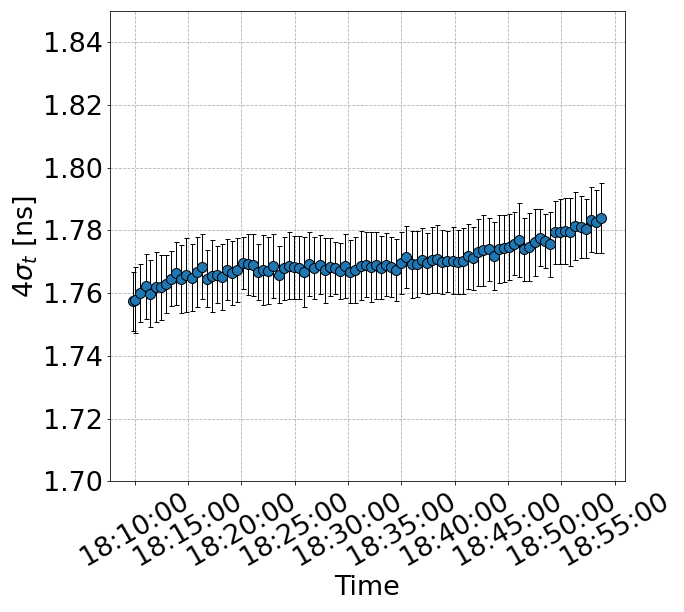
\includegraphics[width=.95\linewidth]{images/app_c/bunch_length_cc_md_sep_coast6.png}  
        \caption{$k_\mathrm{LOD}=-30 \mathrm{/m^{4}}$}
        %\label{fig:cc_md_2022_coast6}
    \end{subfigure}
    \begin{subfigure}{.4\textwidth}
        \centering
        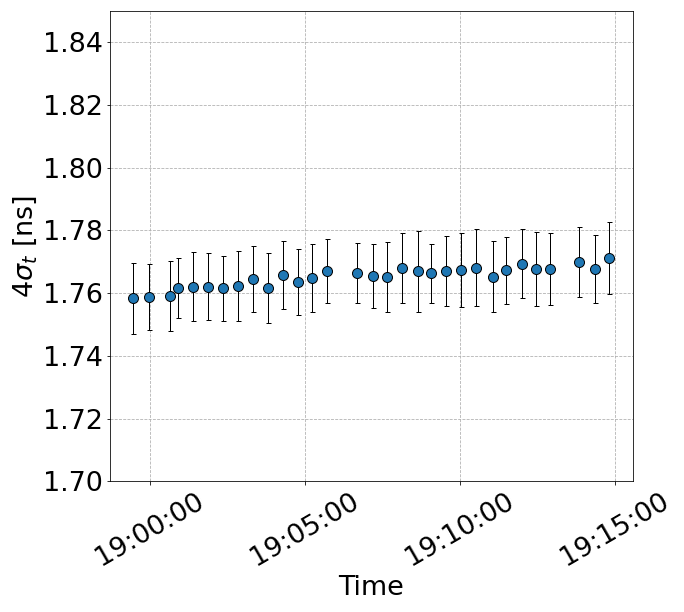
\includegraphics[width=.95\linewidth]{images/app_c/bunch_length_cc_md_sep_coast7.png}  
        \caption{$k_\mathrm{LOD}=-20 \mathrm{/m^{4}}$}
        %\label{fig:cc_md_2022_coast7}
    \end{subfigure}
    \begin{subfigure}{.4\textwidth}
        \centering
        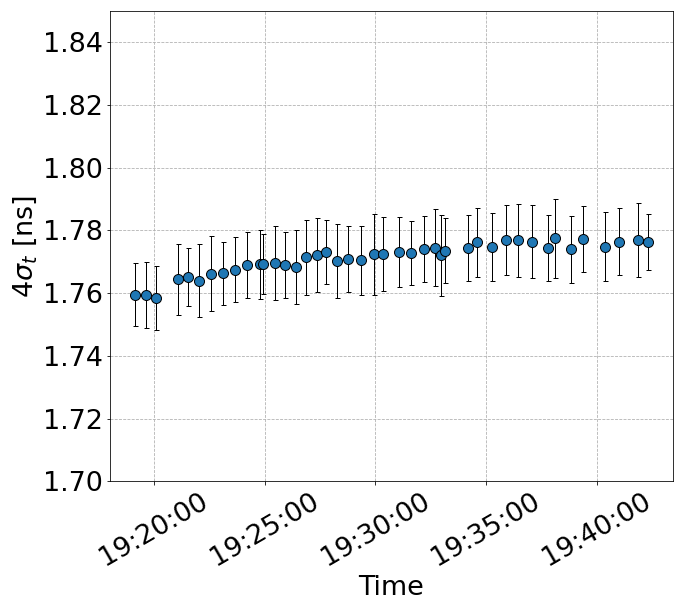
\includegraphics[width=.95\linewidth]{images/app_c/bunch_length_cc_md_sep_coast8.png}  
        \caption{$k_\mathrm{LOD}=-10 \mathrm{/m^{4}}$}
        %\label{fig:cc_md_2022_coast8}
    \end{subfigure}
    \begin{subfigure}{.4\textwidth}
            \centering
            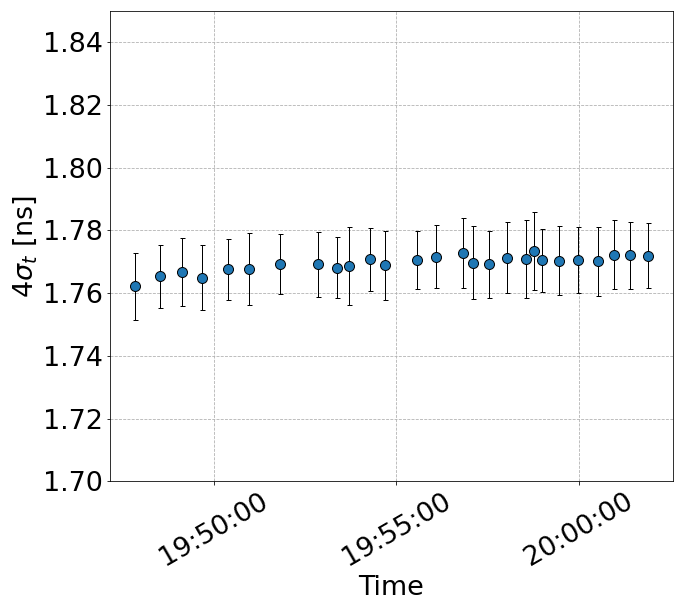
\includegraphics[width=.95\linewidth]{images/app_c/bunch_length_cc_md_sep_coast9.png}  
            \caption{$k_\mathrm{LOD}=+30 \mathrm{/m^{4}}$}
            %\label{fig:cc_md_2022_coast9}
    \end{subfigure}
    \begin{subfigure}{.4\textwidth}
        \centering
        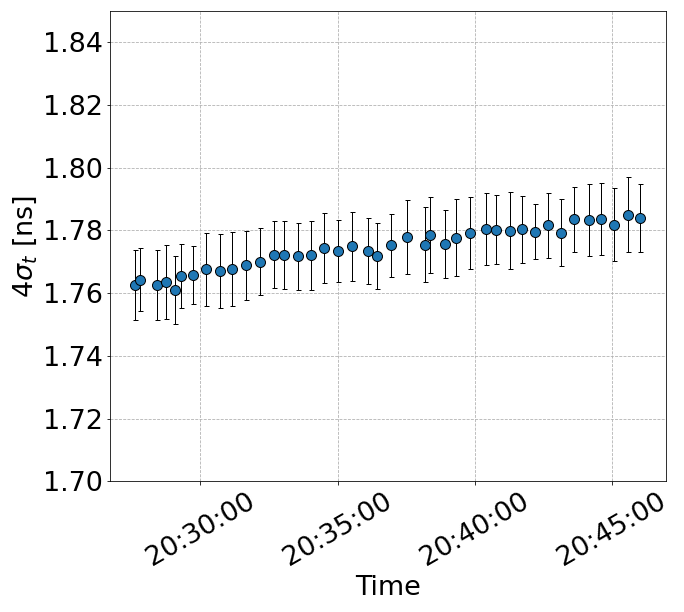
\includegraphics[width=.95\linewidth]{images/app_c/bunch_length_cc_md_sep_coast11.png}  
        \caption{$k_\mathrm{LOD}=+10  \mathrm{/m^{4}}$}
        %\label{fig:cc_md_2022_coast9}
\end{subfigure}
    \caption{Evolution of the bunch length during the CC Experiment III on September 12, 2022. The different octupole settings are displayed at the captions of each plot.}
    \label{fig:cc_md_sep_2022_overview_plots_klod_scan_bunch_length}
 \end{figure}


The average measured bunch length over all above coasts in 2022, was found to be, 4$\sigma_t$=1.77\,ns. 



\newpage

\subsection{Experiment IV: emittance growth measurements driven primarily by amplitude noise}\label{subsec:2022_exp4_bunch_length}

\begin{figure}[h]
    \centering         §
    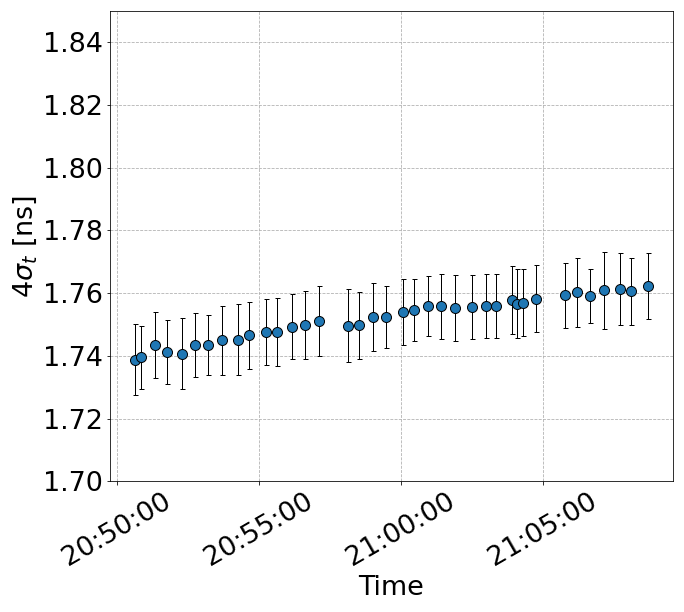
\includegraphics[width=0.6\textwidth]{images/app_e/sps_cc_md_12sep_COAST_12.png}
        \caption{Evolution of the bunch length during the CC Experiment IV on September 12, 2022.}
        \label{fig:bunch_length_exp4}
 \end{figure}
 


The average measured bunch length over the coast was found to be, 4$\sigma_t$=1.75\,ns. 


\newpage
 \section{Intensity measurements}\label{sec:intensity_meas_2022}

 The intensity measurements presented in the section were acquired using the  Beam Current Transformer (in particular with the device SPS.BCTDC.41435) which is installed in the SPS machine. The Beam Current Transformer measures the beam induced current in its ferrite core and transforms it to the number of protons per beam. Fruther details on their working principle and operation can be found in~\cite{Jones:1982418, Jakob:624188}.  


 \subsection{Experiment I: dependece of emittance growth on CC RF noise power}\label{subsec:2022_exp1_intensity}

 % Plotting script: /eos/user/n/natriant/2022/SPS_MDs_2022/cc_md_16May2022/BCTDC_intensity/plot_intensity_evolution.ipynb
 \begin{figure}[htp]
    \centering
    \begin{subfigure}{.45\textwidth}
        \centering
        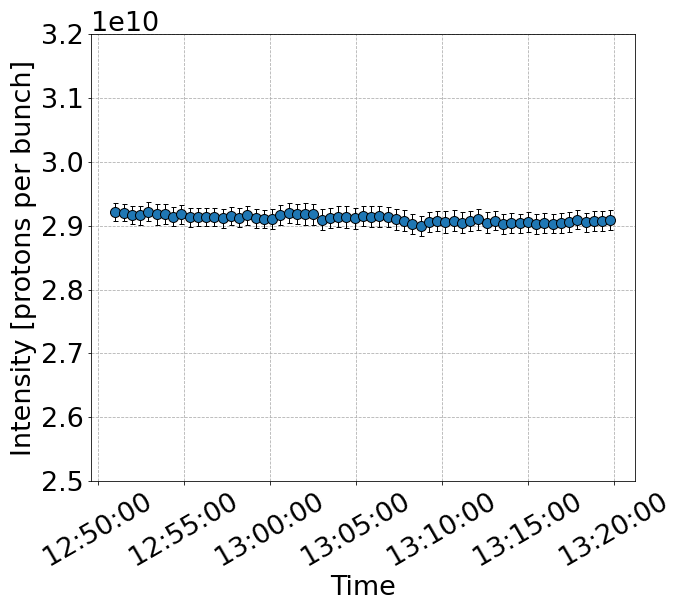
\includegraphics[width=.95\linewidth]{images/app_e/intensity_cc_md_16May22_coast_2.png}  
        \caption{-115.2\,dBc/Hz}
        %\label{fig:cc_md_2022_coast2}
    \end{subfigure}
    \begin{subfigure}{.45\textwidth}
        \centering
        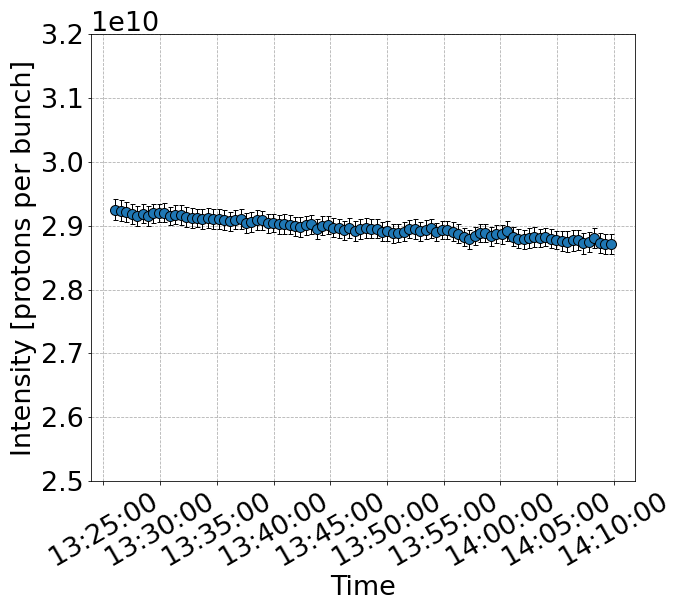
\includegraphics[width=.95\linewidth]{images/app_e/intensity_cc_md_16May22_coast_3.png}  
        \caption{-109.5\,dBc/Hz}
        %\label{fig:cc_md_2022_coast3}
    \end{subfigure}
    \begin{subfigure}{.45\textwidth}
        \centering
        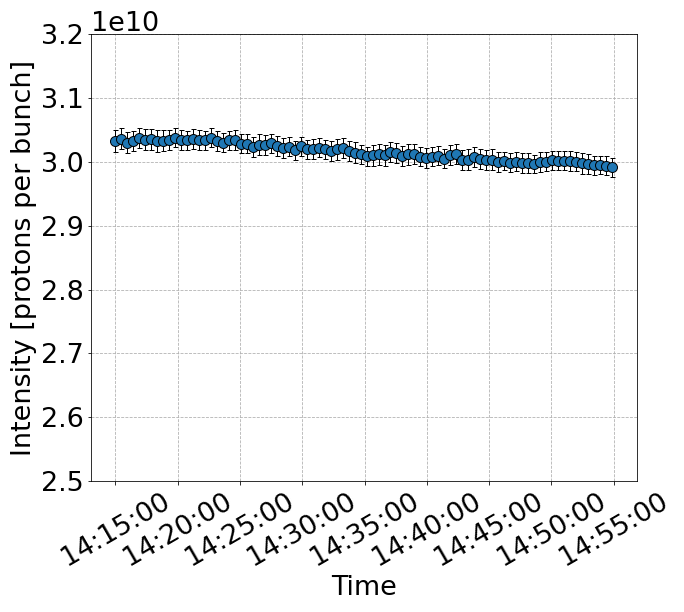
\includegraphics[width=.95\linewidth]{images/app_e/intensity_cc_md_16May22_coast_4.png}  
        \caption{-104.7\,dBc/Hz}
        %\label{fig:cc_md_2022_coast4}
    \end{subfigure}
    \begin{subfigure}{.45\textwidth}
            \centering
            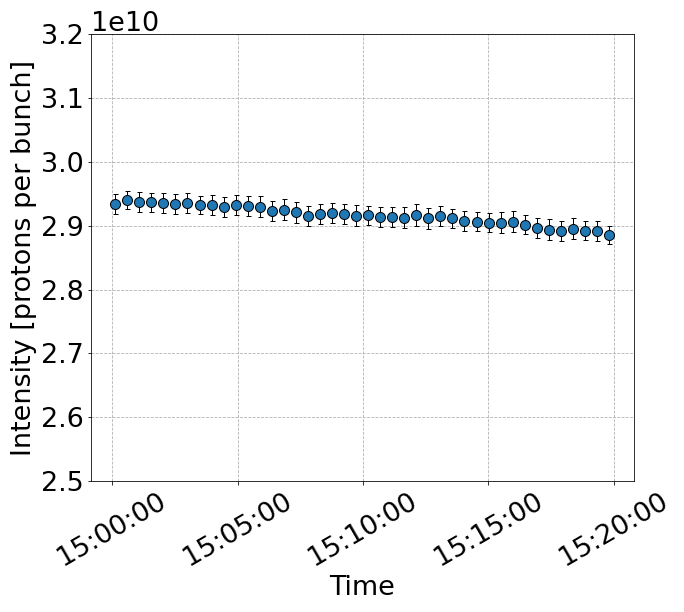
\includegraphics[width=.95\linewidth]{images/app_e/intensity_cc_md_16May22_coast_5.png}  
            \caption{-100.1\,dBc/Hz}
            %\label{fig:cc_md_2022_coast5}
    \end{subfigure}
    \caption{Evolution of the intensity during the CC Experiment I on May 16, 2022. The different phase noise levels injected in the RF system of CC1, are displayed at the captions of each plot.}
    \label{fig:cc_md_16_may_2022_intensity_overview_exper1}
 \end{figure}
 
\newpage
 \subsection{Experiment II: sensitivity of emittance growth to amplitude-dependent tune shift}\label{subsec:2022_exp2_intensity}


 % Plotting script: /eos/user/n/natriant/2022/SPS_MDs_2022/cc_md_16May2022/BCTDC_intensity/plot_intensity_evolution.ipynb
\begin{figure}[htp]
     \centering
     \begin{subfigure}{.45\textwidth}
         \centering
         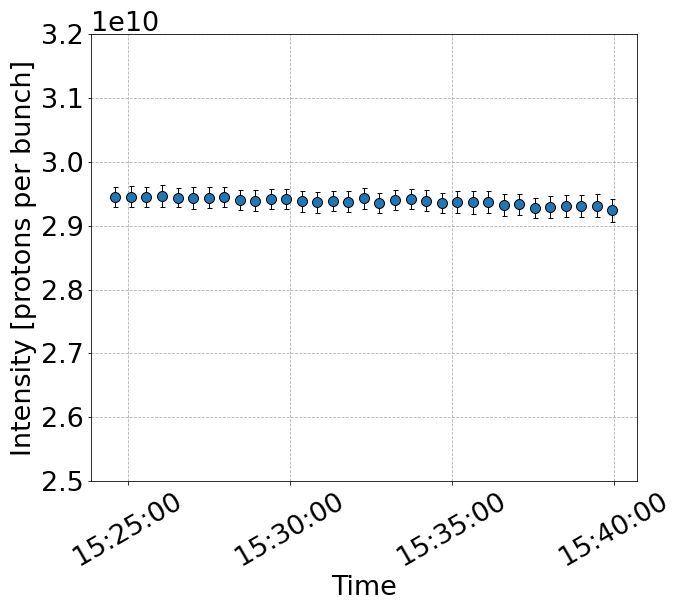
\includegraphics[width=.95\linewidth]{images/app_e/intensity_cc_md_16May22_coast_6.png}  
         \caption{$k_\mathrm{LOD}=+15 \mathrm{/m^{4}}$}
         %\label{fig:cc_md_2022_coast6}
     \end{subfigure}
     \begin{subfigure}{.45\textwidth}
         \centering
         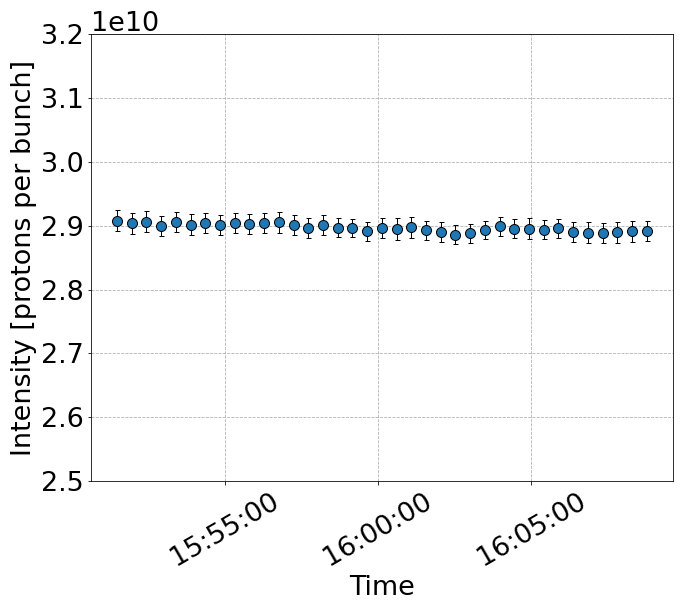
\includegraphics[width=.95\linewidth]{images/app_e/intensity_cc_md_16May22_coast_7.png}  
         \caption{$k_\mathrm{LOD}=+10  \mathrm{/m^{4}}$}
         %\label{fig:cc_md_2022_coast7}
     \end{subfigure}
     \begin{subfigure}{.45\textwidth}
         \centering
         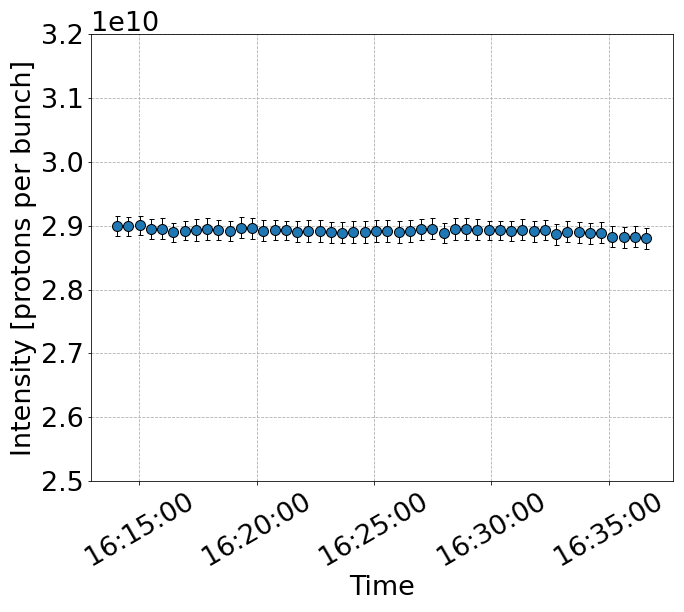
\includegraphics[width=.95\linewidth]{images/app_e/intensity_cc_md_16May22_coast_8.png}  
         \caption{$k_\mathrm{LOD}=+5  \mathrm{/m^{4}}$}
         %\label{fig:cc_md_2022_coast8}
     \end{subfigure}
     \begin{subfigure}{.45\textwidth}
             \centering
             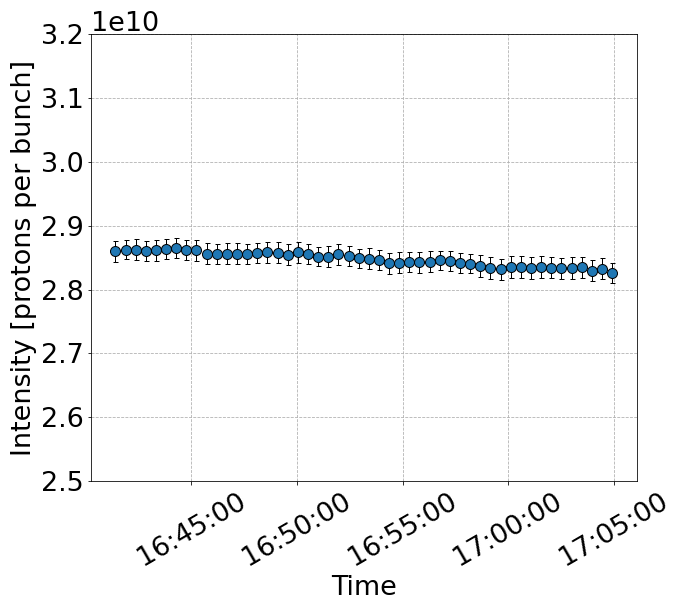
\includegraphics[width=.95\linewidth]{images/app_e/intensity_cc_md_16May22_coast_9.png}  
             \caption{$k_\mathrm{LOD}=-5 \mathrm{/m^{4}}$}
             %\label{fig:cc_md_2022_coast9}
     \end{subfigure}
     \caption{Evolution of the intensity during the  CC Experiment II on May 16, 2022. The different octupole settings are displayed at the captions of each plot.}
     \label{fig:cc_md_2022_overview_plots_klod_scan_intensity_exper2}
\end{figure}


 The average measured intensity over all above coasts on May 16, 2022 (Experiment III) was found to be 2.9$\times 10^{10}$\,protons per bunch. 
 
\newpage
 \subsection{Experiment III: emittance growth measurements in the presence of strong octupoles}\label{subsec:2022_exp3_intensity}

 \begin{figure}[htp]
    \centering
    \begin{subfigure}{.4\textwidth}
        \centering
        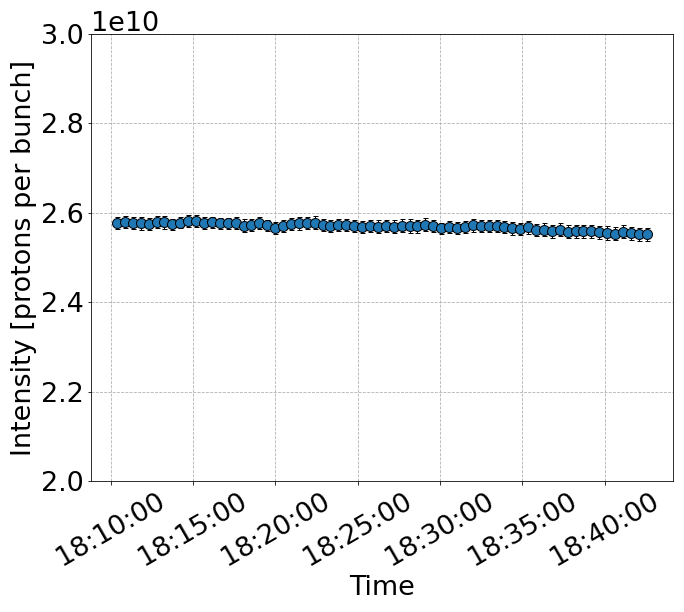
\includegraphics[width=.95\linewidth]{images/app_e/intensity_cc_md_12Sep22_coast_6.png}  
        \caption{$k_\mathrm{LOD}=-30 \mathrm{/m^{4}}$}
        %\label{fig:cc_md_2022_coast6}
    \end{subfigure}
    \begin{subfigure}{.4\textwidth}
        \centering
        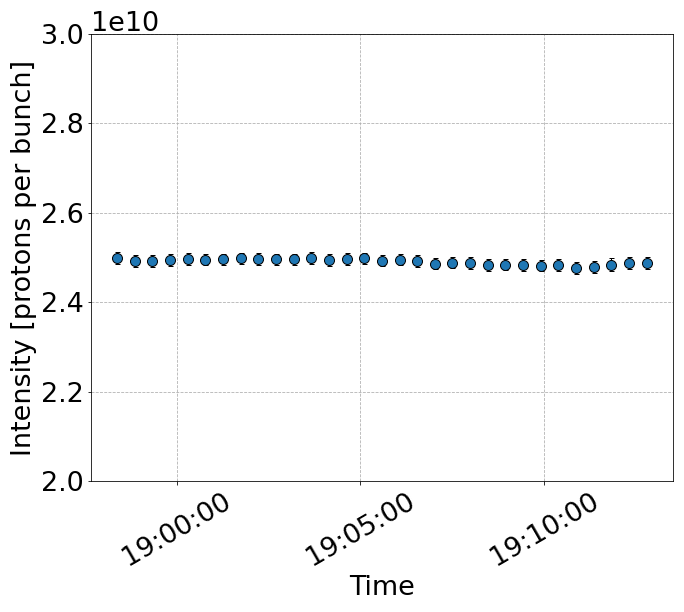
\includegraphics[width=.95\linewidth]{images/app_e/intensity_cc_md_12Sep22_coast_7.png}  
        \caption{$k_\mathrm{LOD}=-20 \mathrm{/m^{4}}$}
        %\label{fig:cc_md_2022_coast7}
    \end{subfigure}
    \begin{subfigure}{.4\textwidth}
        \centering
        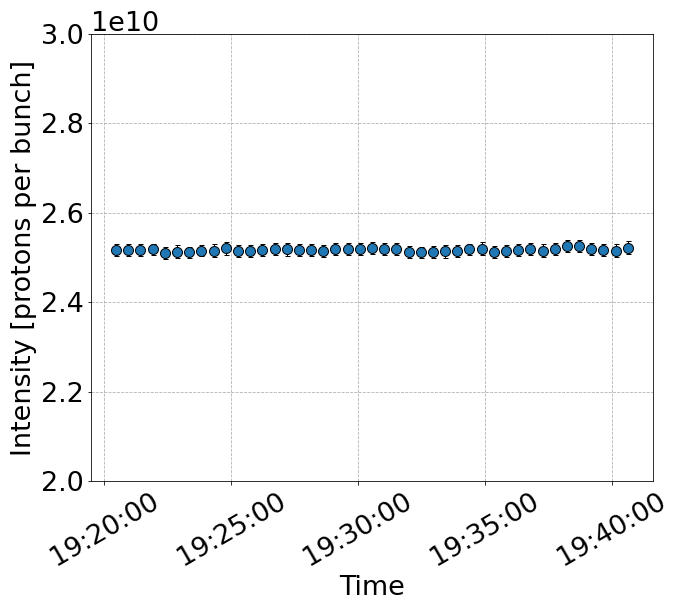
\includegraphics[width=.95\linewidth]{images/app_e/intensity_cc_md_12Sep22_coast_8.png}  
        \caption{$k_\mathrm{LOD}=-10 \mathrm{/m^{4}}$}
        %\label{fig:cc_md_2022_coast8}
    \end{subfigure}
    \begin{subfigure}{.4\textwidth}
            \centering
            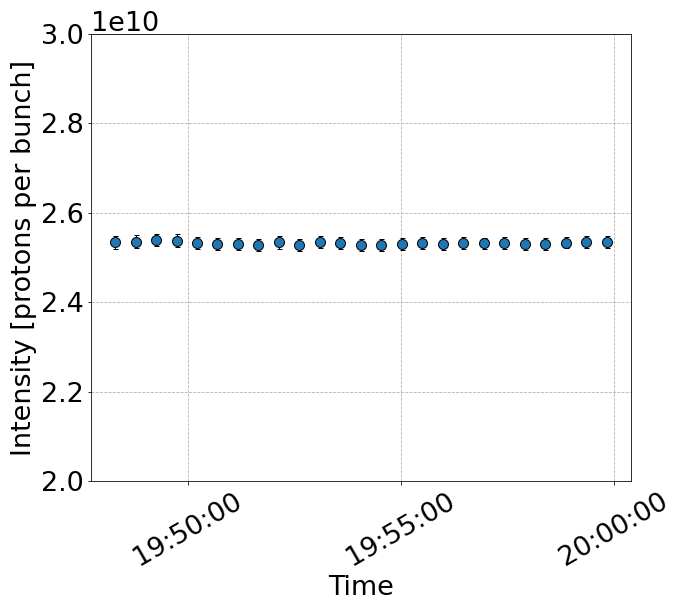
\includegraphics[width=.95\linewidth]{images/app_e/intensity_cc_md_12Sep22_coast_9.png}  
            \caption{$k_\mathrm{LOD}=+30 \mathrm{/m^{4}}$}
            %\label{fig:cc_md_2022_coast9}
    \end{subfigure}
    \begin{subfigure}{.4\textwidth}
        \centering
        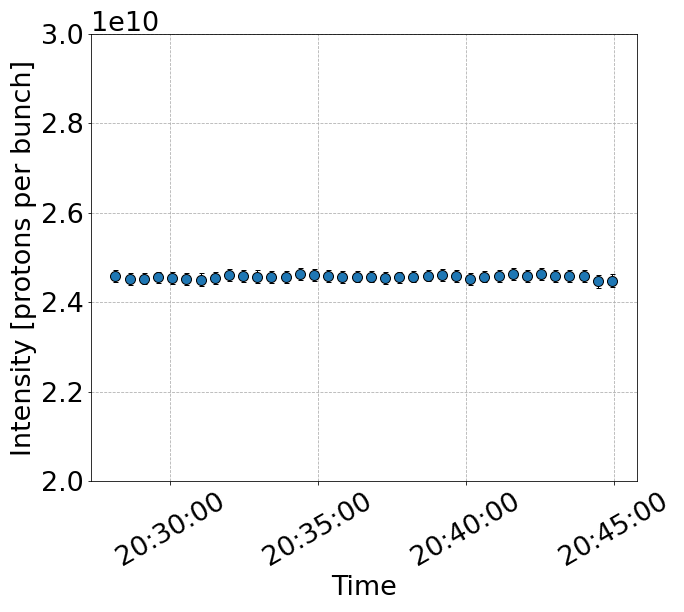
\includegraphics[width=.95\linewidth]{images/app_e/intensity_cc_md_12Sep22_coast_11.png}  
        \caption{$k_\mathrm{LOD}=+10  \mathrm{/m^{4}}$}
        %\label{fig:cc_md_2022_coast9}
\end{subfigure}
    \caption{Evolution of the inensity during the CC Experiment III on September 12, 2022. The different octupole settings are displayed at the captions of each plot.}
    \label{fig:cc_md_sep_2022_overview_plots_klod_scan_intensity}
 \end{figure}

 The average measured intensity over all above coasts on September 12, 2022 (Experiments III) was found to be 2.5$\times 10^{10}$\,protons per bunch. 

\newpage


\subsection{Experiment IV: emittance growth measurements driven primarily by amplitude noise}\label{subsec:2022_exp4_intensity}

\begin{figure}[h]
    \centering         §
    \includegraphics[width=0.6\textwidth]{images/app_e/intensity_cc_md_12Sep22_coast_12.png}
        \caption{Evolution of the intensity during the CC Experiment IV on September 12, 2022.}
        \label{fig:bunch_length_exp4}
 \end{figure}
 


The average intensity over the coast was found to be, 2.4$\times 10^{10}$ protons per bunch. 
